\section{The de Bruijn Newman flow from the P\'olya density}\label{ch:dbn}

Li's criterion reads RH from Taylor data at one point, and it tests one fixed Thorin functional against a sequence of test functions (Section~\ref{ch:li}). The de Bruijn Newman flow reads RH from a deformation of the P\'olya kernel, and so deforms the functional instead. Multiplying the kernel by a Gaussian factor turns $\Xi$ into a family of entire functions $H_t$ that evolve by the backward heat equation. RH says that $H_0$ has only real zeros, and the de Bruijn Newman constant $\Lambda$ is defined by the property that $H_t$ has only real zeros exactly when $t\ge\Lambda$. In Thorin terms the flow is a path of clocks that are generalised gamma convolutions for $t\ge\Lambda$ (Theorem~\ref{rz:thm:dbn}), and RH says that the path stays in this class down to $t=0$. The P\'olya route computes $H_t$ at the cost of $\Xi$, since the Gaussian factor only multiplies the node values. We follow two pairs of zeros backward in time to their collisions, the closest pair below height $200$ and Lehmer's pair near height $7005$, and compare the collision times with the isolated pair estimate and with the lower bound of Csordas, Smith and Varga. The Stieltjes moment test of Section~\ref{ch:heat} runs along the flow at the cost of its moments, and a Hankel test of finite order turns out to be a window on the low zeros that registers their collisions one at a time. Biane's description of the free convolution with a semicircle law singles out Laguerre's quantity $-(\log H_0)''$, which predicts the collision times from $H_0$ alone and, with corrections computed along the flow, brackets each of them.

\subsection{The flow, the motion of its zeros and its Thorin form}\label{sec:ch21:flow}

In the normalisation of Rodgers and Tao \cite{RodgersTao}, which Theorem~\ref{rz:thm:dbn} also uses,
\begin{gather*}
H_t(z)=\int_0^\infty e^{tu^2}\Phi_{\rm dBN}(u)\cos(zu)\,du,\\
\Phi_{\rm dBN}(u)=\sum_{n\ge1}\big(2\pi^2n^4e^{9u}-3\pi n^2e^{5u}\big)\exp(-\pi n^2e^{4u}),
\end{gather*}
so that $H_0(z)=\frac18\Xi(z/2)$. If $v=2u$ denotes the variable of \eqref{eq:ch2:Phi}, then $\Phi_{\rm dBN}(u)=\frac12\Phi(v)$ and
\[
8H_t(2\theta)=\int_{\mathbb R}\Phi(v)\,e^{tv^2/4}\cos(\theta v)\,dv,
\]
so the flow multiplies the kernel of \eqref{eq:ch2:Phi} by $e^{tv^2/4}$, and a zero $z$ of $H_t$ corresponds to the ordinate $\theta=z/2$.

De Bruijn showed that $H_t$ has only real zeros for $t\ge\frac12$ and that the property persists forward in time \cite{deBruijn}. Newman showed that there is a constant $\Lambda>-\infty$, at most $\frac12$ by de Bruijn's theorem, such that $H_t$ has only real zeros exactly for $t\ge\Lambda$, and conjectured $\Lambda\ge0$ \cite{Newman1976}, which Rodgers and Tao proved \cite{RodgersTao}. Ki, Kim and Lee sharpened de Bruijn's bound to $\Lambda<\frac12$ \cite{KKL09}, the Polymath project proved $\Lambda\le0.22$ \cite{Polymath}, and Platt and Trudgian improved this to $\Lambda\le0.2$ \cite{PT21}. De Bruijn's bound comes from a theorem about strips: if the zeros of $H_0$ lie in $|\im z|\le\Delta$, then $H_t$ has only real zeros for $t\ge\Delta^2/2$ \cite[Theorem 13]{deBruijn}, and the critical strip gives $\Delta=1$. A zero free half plane $\re s>\alpha$ gives $\Delta=2\alpha-1$, hence $\Lambda\le2(\alpha-\frac12)^2$; for the half plane $\re s>\frac78$ announced in October 2026 (Section~\ref{sec:ch25:open}) this is $\Lambda\le\frac9{32}$, weaker than $0.2$, which a zero free half plane improves only if $\alpha<\frac12+\sqrt{0.1}\approx0.816$. RH is the inequality $\Lambda\le0$, so by the theorem of Rodgers and Tao it is equivalent to $\Lambda=0$: if RH holds, the zeros of $H_t$ are all real from $t=0$ on and at no earlier time.

While the zeros are simple they move according to
\[
\frac{dz_k}{dt}=2\sum_{j\ne k}\frac1{z_k-z_j},
\]
the sum running over all other zeros, positive and negative, with $z_j$ and $-z_j$ taken together. Differentiating $H_t(z_k(t))=0$ in $t$ and using the backward heat equation $\partial_tH_t=-\partial_z^2H_t$ gives $dz_k/dt=\partial_z^2H_t/\partial_zH_t$ at $z_k$, and the Hadamard product of the even function $H_t$ turns this into the display (Exercise~\ref{ex:ch21:motion}). The equation is the gradient flow of unit charges on the line with logarithmic interaction, so forward in time the zeros repel each other, spread and become more regular. Backward in time neighbouring zeros approach each other, and a close pair collides and then leaves the real axis as a conjugate pair. A pair at distance $D$ that is isolated from the other zeros obeys $dD/dt\approx4/D$, so $D^2\approx D_0^2+8t$ with $D_0=D(0)$, and the pair collides at $t\approx-D_0^2/8$. RH is the statement that no two zeros collide at a positive time.

Let $R_t(u)=H_t(0)/H_t(2i\sqrt u)$, where $u$ is the variable of the clock (written $s$ in Chapters~\ref{chap:rzeta} and \ref{chap:rzid}), not the variable of integration in $H_t$, so that $R_0$ is the clock $1/G$. By Theorem~\ref{rz:thm:dbn}, for every $t\ge\Lambda$, and so for every $t\ge0.2$, $R_t$ is the Laplace transform of a GGC with Thorin measure $\sum_k\delta_{(z_k(t)/2)^2}$, where $z_k(t)$ runs over the positive zeros of $H_t$: along the path of clocks the Thorin atoms move with the zeros. The Thorin density at resolution $\varepsilon$ follows the flow in the same way. Put $\xi_t(s)=8H_t\big(-2i(s-\frac12)\big)$, so that $\xi_t(\frac12+i\theta)=8H_t(2\theta)$ and $\xi_0=\xi$, and
\[
\rho_{\varepsilon,t}(\theta)=\pi^{-1}\re(\xi_t'/\xi_t)\big(\tfrac12+\varepsilon+i\theta\big).
\]
Each zero $z$ of $H_t$ gives the zero $\frac12+iz/2$ of $\xi_t$, and for every $t$ the function $\rho_{\varepsilon,t}$ is the sum of the Poisson kernels $P_{\frac12+\varepsilon-\beta}(\theta-\gamma)$ over the zeros $\beta+i\gamma$ of $\xi_t$. For $t\ge\Lambda$ every $\beta$ equals $\frac12$ and $\rho_{\varepsilon,t}$ is the Thorin density of $R_t$ at resolution $\varepsilon$; the P\'olya route computes it by the same multiplication of the node values. As $t$ decreases through a collision, $\rho_{\varepsilon,t}$ shows the off line signature of Section~\ref{ch:offline}: two Poisson peaks merge, and after the collision the pair contributes the kernels $P_{\varepsilon+d(t)}+P_{\varepsilon-d(t)}$ at its ordinate, where $d(t)$, half the imaginary part of the pair in $z$, grows from zero; the second kernel is negative once $d(t)>\varepsilon$. The flow thus produces off line configurations of known geometry, on which the diagnostics of Chapters~\ref{chap:measure} to \ref{chap:heat} can be calibrated; Section~\ref{sec:open:calib} lists this calibration among the open computations.

\subsection{Two collisions computed from the P\'olya kernel}\label{sec:ch21:collisions}

The P\'olya route evaluates $H_t$ at any $t$ by multiplying the node values $\Phi(v_j)$ by $e^{tv_j^2/4}$ and summing. The factor is entire, so the error analysis of Section~\ref{ch:polya} carries over, and for $|t|\le1$ the factor is at most $e^{9/4}$ on the truncation interval $|v|\le3$. Among the $79$ zeros below height $200$ the closest pair is $\gamma_{71}=184.8745$, $\gamma_{72}=185.5988$, at distance $0.7243$ in $\theta$, that is $D_0=1.4486$ in $z$. We follow the pair by the sign changes of $H_t(2\theta)$ at $121$ equally spaced points of $[\gamma_{71}-0.3,\gamma_{72}+0.3]$, computed at $420$ bits, and refine each zero by Newton's method; Table~\ref{tab:ch21:traj} and Figure~\ref{fig:ch21:dbn} show the result.

\begin{table}[htbp]
\centering\small
\begin{tabular}{rll}
\toprule
$t$ & zeros in $\theta=z/2$ & sign changes\\
\midrule
0.2 & 184.676, 185.590 & 2\\
0.1 & 184.771, 185.598 & 2\\
0.0 & 184.874, 185.599 & 2\\
$-0.05$ & 184.931, 185.595 & 2\\
$-0.1$ & 184.992, 185.587 & 2\\
$-0.15$ & 185.059, 185.573 & 2\\
$-0.2$ & 185.136, 185.550 & 2\\
$-0.3$ & none & 0\\
\bottomrule
\end{tabular}
\caption{The closest pair below height $200$ under the de Bruijn Newman flow, located by the sign changes on a grid of step $0.011$ and refined by Newton's method; $t$ is the de Bruijn Newman time.}
\label{tab:ch21:traj}
\end{table}

Bisection on $t$ for the disappearance of the two sign changes gives the collision time
\[
t_*=-0.2880,
\]
with a grid error of at most $6.1\times10^{-5}$. Near a collision the term $4/D$ dominates the motion of the pair, so $D^2\approx8(t-t_*)$ and the gap in $\theta$ is about $\sqrt{2(t-t_*)}$; on a grid of step $h$ the sign changes therefore vanish at a time at most $h^2/2$ above $t_*$. The isolated pair estimate is $-D_0^2/8=-0.262$: the neighbouring zeros, which the estimate ignores, delay the collision. Since nonreal zeros persist backward in time, $H_t$ has nonreal zeros for every $t$ below the collision time, so $\Lambda\ge t_*\approx-0.288$; this numerical lower bound is far weaker than the published bounds, as expected for a pair of ordinary spacing.

\begin{figure}[htbp]
\centering
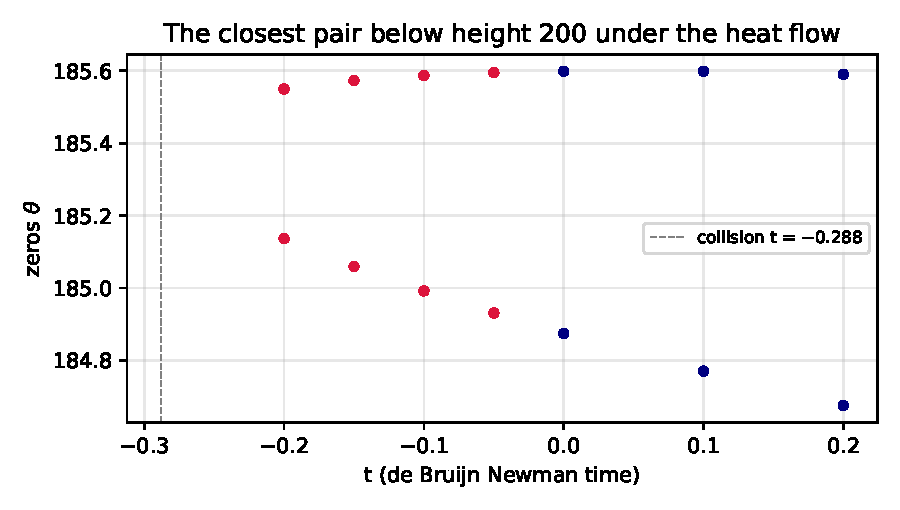
\includegraphics[width=0.7\textwidth]{fig/dbn.pdf}
\caption{Zeros of the closest pair below height $200$ along the de Bruijn Newman flow, refined by Newton's method as in Table~\ref{tab:ch21:traj}, for $t\ge0$ and $t<0$, and the computed collision time (dashed line).}
\label{fig:ch21:dbn}
\end{figure}

Lehmer's pair near height $7005$, $\gamma_{6709}=7005.0629$ and $\gamma_{6710}=7005.1006$ (Section~\ref{sec:ch5:lehmer}), is much closer: $D_0=2\times0.0377=0.0754$, and its isolated pair estimate $-D_0^2/8=-7.1\times10^{-4}$ is about $400$ times closer to zero than the collision time of the pair below height $200$. The tilted P\'olya route evaluates $H_t$ at that height at the same cost as $\Xi$, with the Gaussian factor $e^{tv^2/4}$ included in the exponential at each complex node $v=x+i\eta$. With the parameters of Section~\ref{sec:ch5:lehmer} ($\delta=0.01$, $256$ bits, $13001$ nodes) we track the two sign changes of the pair on a grid of step $0.0025$ in $\theta$ over $[7005.03,7005.13]$. Both sign changes are present at $t=0$ and absent at $t=-0.004$, and twelve bisection steps on this interval give $-7.10\times10^{-4}$, which by the argument above lies above the collision time by at most $0.0025^2/2\approx3\times10^{-6}$. Newton's method for the double zero, $H_t(2\theta)=\partial_\theta H_t(2\theta)=0$ in the unknowns $\theta$ and $t$, started from this value, gives
\[
t_*=-7.11\times10^{-4}
\]
at $\theta=7005.0817$, and Figure~\ref{fig:ch21:lehmerflow} shows the collision. Here the isolated pair estimate is accurate: for a pair this close the neighbours hardly matter, whereas for the ordinary pair below height $200$ they moved the collision from $-0.262$ to $-0.288$. The computation takes about half a minute, and the numerical lower bound $\Lambda\ge t_*$ that it gives is much sharper than the one from the pair below height $200$.

\begin{figure}[htbp]
\centering
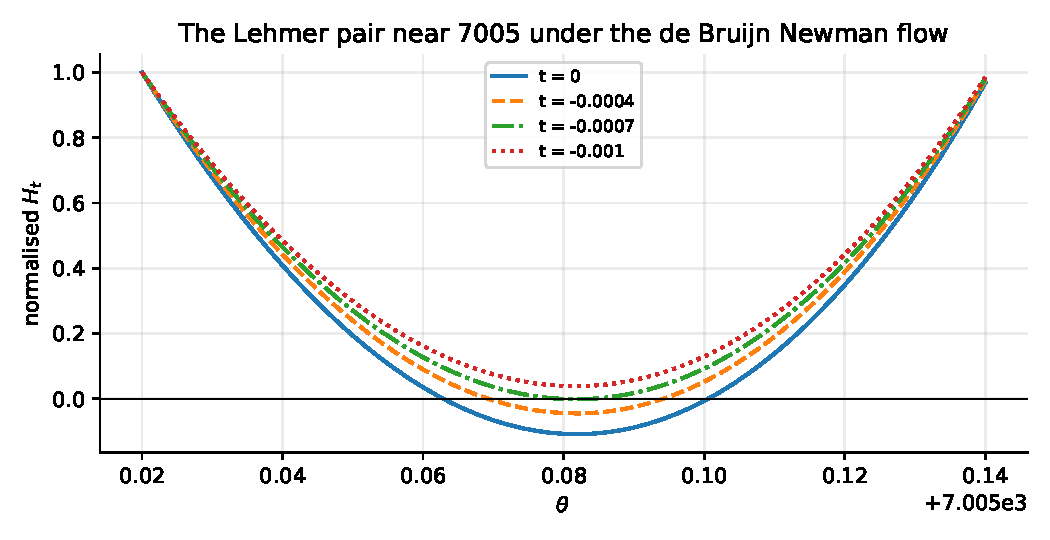
\includegraphics[width=0.8\textwidth]{fig/lehmerflow.pdf}
\caption{The function $\theta\mapsto H_t(2\theta)e^{\pi\theta/4}$ near the Lehmer pair at height $7005$, divided by its maximum absolute value on the window, for four times of the de Bruijn Newman flow, computed with the tilted P\'olya route. At $t=0$ it has two sign changes; at $t=-7\times10^{-4}$, slightly above the collision time $-7.11\times10^{-4}$, they nearly coincide; at $t=-10^{-3}$ the pair has left the real axis.}
\label{fig:ch21:lehmerflow}
\end{figure}

P\'olya's function $K_{i\theta/2}(2\pi)$ behaves differently under the same flow. Down to $t=-60$ none of its real zeros below height $90$ collide, and as $t$ decreases from $0$ to $-0.5$ they rise almost as a rigid block, at speeds within $2\%$ of the mean speed $\pi/8$ that the two functions share, while the zeros of $\Xi$ rise at speeds between $0.004$ and $0.735$; yet by Newman's theorem the de Bruijn Newman constant of P\'olya's function is finite (Section~\ref{sec:biane:flow}).

\subsection{The Hankel test along the flow}\label{sec:ch21:hankel}

The Stieltjes moment test of Section~\ref{ch:heat} (Table~\ref{tab:ch12:jacobi}) needs only the Taylor coefficients of $\Xi$ at the centre, and along the flow these are moments of the reweighted kernel \cite{P26wig}. Putting $\theta=i\sqrt u$ in the formula for $8H_t(2\theta)$ of Section~\ref{sec:ch21:flow} gives
\[
G_t(u)=\frac{H_t(2i\sqrt u)}{H_t(0)}=\sum_{k\ge0}\frac{M_k(t)\,u^k}{(2k)!\,M_0(t)},\qquad M_k(t)=\int_{\mathbb R}v^{2k}e^{tv^2/4}\Phi(v)\,dv,
\]
and $G_0$ is the function $G$ of Section~\ref{ch:heat}. Write $\pm\theta_j(t)$ for the zeros of $\theta\mapsto H_t(2\theta)$, so that $\theta_j(0)=\gamma_j$ while the zeros are on the line. Since $H_t$ is even and entire of order one, $G_t$ has order $\frac12$ and $G_t(u)=\prod_j(1+u/a_j(t))$ with $a_j(t)=\theta_j(t)^2$, so the Newton identities turn the $M_k(t)$ into the moments $m_n(t)=\sum_ja_j(t)^{-n-1}$, exactly as at $t=0$. If every $\theta_j(t)$ is real, the $m_n(t)$ are the moments of the positive measure $\nu_t=\sum_ja_j(t)^{-1}\delta_{1/a_j(t)}$, and every Hankel matrix $\mathcal H_N(t)=[m_{i+j}(t)]_{i,j<N}$ is positive definite. The converse is proved as at $t=0$: if every $\mathcal H_N(t)$ is positive definite, every $a_j(t)$ is real, and it is positive because $H_t$ has no zeros on the imaginary axis: $H_t(iy)=\int_0^\infty e^{tu^2}\Phi_{\rm dBN}(u)\cosh(yu)\,du>0$, the kernel \eqref{eq:ch2:Phi} being strictly positive. So at every time $t$ all the matrices $\mathcal H_N(t)$ are positive definite exactly when $H_t$ has only real zeros, that is, when $t\ge\Lambda$. Each $M_k(t)$ is one sum over the node values of $\Phi$, reweighted by $e^{tv^2/4}$, and the Cholesky factor gives the Jacobi matrix $J_N(t)$, whose eigenvalues return the lowest zeros of $H_t$ as $J_N$ returns the $\gamma_j$ at $t=0$ (Table~\ref{tab:ch21:flowzeros}).

\begin{table}[htbp]
\centering\small
\begin{tabular}{rlllll}
\toprule
$t$ & $\theta_1(t)$ & $\theta_2(t)$ & $\theta_3(t)$ & $\theta_5(t)$ & $\theta_{10}(t)$\\
\midrule
$0.2$ & 14.07681 & 20.94669 & 24.95221 & 32.88801 & 49.72988\\
$0$ & 14.13473 & 21.02204 & 25.01086 & 32.93506 & 49.77383\\
$-0.4$ & 14.25083 & 21.17365 & 25.12774 & 33.02595 & 49.85213\\
$-1.0$ & 14.42563 & 21.40341 & 25.30189 & 33.15277 & 49.93350\\
\bottomrule
\end{tabular}
\caption{Zeros $\theta_n(t)$ of $\theta\mapsto H_t(2\theta)$ returned by the Jacobi matrix $J_{30}(t)$ of the moments $m_0(t),\dots,m_{59}(t)$; at $t=0$ they are $\gamma_1$, $\gamma_2$, $\gamma_3$, $\gamma_5$ and $\gamma_{10}$. At each of the four times $J_{30}(t)$ returns $\theta_1(t),\dots,\theta_{12}(t)$ to within $3.1\times10^{-7}$ of the zeros that Newton's method finds on $H_t$, and $\theta_{13}(t)$ only to within $5.2\times10^{-4}$. Backward in time each of these zeros moves up.}
\label{tab:ch21:flowzeros}
\end{table}

Going back from $t=0$, the matrix $\mathcal H_N(t)$ stays positive definite until a time $t^*_N$ at which it ceases to be. Since $\mathcal H_N(t)$ is the leading block of $\mathcal H_{N+1}(t)$, $t^*_N\le t^*_{N+1}$. Under RH every $t^*_N$ is negative, because $\mathcal H_N(0)$ is positive definite, and $t^*_N\to0$: for each $t<0$ the function $H_t$ has nonreal zeros by the theorem of Rodgers and Tao, so some $\mathcal H_N(t)$ is not positive definite, and then $t^*_{N'}\ge t$ for every $N'\ge N$. With the moments from the trapezoid rule of step $1/600$ on $[0,3.6]$ at $100+16N$ digits (Table~\ref{tab:ch12:jacobi} gives the precision that order $N$ needs at $t=0$), the grid $t=0,-0.05,\dots,-4$ and bisection to $10^{-7}$ give no failure of order $10$ down to $t=-4$, and
\begin{gather*}
t^*_{20}=-1.8991865,\qquad t^*_{30}=-1.2853067,\\
t^*_{40}=-1.2760788,\qquad t^*_{50}=-1.0325048;
\end{gather*}
for $N=30$ a second discretisation (step $1/550$, $650$ digits) gives a bracket that overlaps the first in $[-1.28530669,-1.28530664]$.

Each failure registers a collision. We follow the real zeros of $H_t$ that start at $2\gamma_j$, $j\le64$, back to $t=-2.05$ by the equation of motion of Section~\ref{sec:ch21:flow}, with Newton's method on the trapezoid sum for $H_t$ at each step ($110$ digits, step $1/100$), and locate each collision as a double zero, $H_t(z)=\partial_zH_t(z)=0$, by Newton's method in the two unknowns $z$ and $t$; the backward heat equation, which holds exactly for the trapezoid sum, gives the derivatives in $t$. Thirteen of the pairs below index $59$ collide in this time range, among them those that start at $(\gamma_k,\gamma_{k+1})$ for $k=9$, $13$, $19$, $24$, $27$ and $34$, at
\[
t=-1.87791,\ -1.28527,\ -1.27554,\ -1.14387,\ -0.88108,\ -0.38456
\]
and the heights $\theta=49.664$, $60.491$, $77.027$, $88.466$, $95.540$ and $111.638$; the other seven start at $k=40$, $43$, $45$, $48$, $51$, $53$ and $57$. To see which collision a failure registers, we continue each double zero into the complex plane, starting from $z_c\pm i\sqrt{2(t_c-t)}$ near the collision, and remove the contribution $2\re\theta^{-2n-2}$ of the conjugate pair $\theta=z/2$, $\bar\theta$ from $m_n(t)$. At $t^*_N-\delta$, with $\delta=0.01$ (for $N=40$, $\delta=0.0046$, half the time to the collision of $(\gamma_{13},\gamma_{14})$), the only one of the thirteen pairs whose removal makes $\mathcal H_N(t)$ positive definite again is the one that starts at $(\gamma_9,\gamma_{10})$ for $N=20$, at $(\gamma_{13},\gamma_{14})$ for $N=30$, at $(\gamma_{19},\gamma_{20})$ for $N=40$ and at $(\gamma_{27},\gamma_{28})$ for $N=50$. The same holds at $t^*_N-10^{-5}$, except that there removing $(\gamma_{34},\gamma_{35})$ also restores the order $50$ matrix. The failures thus come $0.021$, $3.7\times10^{-5}$, $5.3\times10^{-4}$ and $0.151$ after the collisions they register.

A Hankel test of finite order is thus a window on the low part of the spectrum. The order $30$ matrix is positive definite at $t=-1.276,-1.278,\dots,-1.284$ and $-1.2852$, after the collision of $(\gamma_{19},\gamma_{20})$ at $-1.27554$ and before that of $(\gamma_{13},\gamma_{14})$ at $-1.28527$: it passes the pair that is too high and too light for its order and registers the lower one. A conjugate pair at height $\theta$ enters $m_n(t)$ with weight of order $\theta^{-2n-2}$, against $\theta_1(t)^{-2n-2}$ for the lowest zero, as at $t=0$, and increasing the order widens the window.

The whole curve $N\mapsto t^*_N$ up to $N=50$ follows from one elimination per time. Let $n_{\rm fail}(t)$ be the index of the first nonpositive pivot of Gaussian elimination on $\mathcal H_{50}(t)$, that is, the least $N\le50$ for which $\mathcal H_N(t)$ is not positive definite, so that $t^*_N=\sup\{t<0:n_{\rm fail}(t)\le N\}$. On the grid of step $0.01$ it is a staircase \cite{P26wig}: no order up to $50$ fails on $[-1.03,0]$, and then $n_{\rm fail}$ is $50$ on $[-1.14,-1.04]$, $46$ on $[-1.18,-1.15]$, $45$ on $[-1.27,-1.19]$, and $39$, $28$ and $27$ at $t=-1.28$, $-1.29$ and $-1.30$ (Table~\ref{tab:ch21:nfail}). To see what each step registers, the table gives, at one time on each step, the least order at which each complex pair breaks the test alone, that is, with the contributions of all the other complex pairs removed from the moments. A pair alone breaks the test at a definite order, a higher pair at a higher order, and $n_{\rm fail}$ is close to the least of these orders. The order at which a pair is seen falls as the pair moves away from the axis: $(\gamma_{27},\gamma_{28})$, which collides at $-0.881$, breaks order $50$ at $t=-1.09$, order $45$ at $-1.16$ and $-1.23$, order $41$ at $-1.28$ and order $39$ at $-1.29$, and $(\gamma_{34},\gamma_{35})$, which collides earlier, at $-0.385$, but lies higher, breaks the test only from $t=-1.28$ on, at order $50$ and then $47$. Removing the pair with the least order moves $n_{\rm fail}$ up to about the next one: at $t=-1.30$ from $27$ to $35$, when $(\gamma_{13},\gamma_{14})$ is removed, at $-1.28$ from $39$ to $41$, when $(\gamma_{19},\gamma_{20})$ is removed, and at $-1.09$ from $50$ to no failure, when $(\gamma_{27},\gamma_{28})$ is removed. With all thirteen pairs removed, no order up to $50$ fails at any of these times.

\begin{table}[htbp]
\centering\small
\begin{tabular}{llrrrrrr}
\toprule
& & & \multicolumn{5}{c}{order broken by $(\gamma_k,\gamma_{k+1})$ alone}\\
\cmidrule(l){4-8}
$t$ & $n_{\rm fail}(t)$ & at $t=$ & $k=13$ & $19$ & $24$ & $27$ & $34$\\
\midrule
$[-1.03,0]$ & none & & & & & & \\
$[-1.14,-1.04]$ & $50$ & $-1.09$ & real & real & real & $50$ & $>50$\\
$[-1.18,-1.15]$ & $46$ & $-1.16$ & real & real & $44$ & $45$ & $>50$\\
$[-1.27,-1.19]$ & $45$ & $-1.23$ & real & real & $44$ & $45$ & $>50$\\
$-1.28$ & $39$ & $-1.28$ & real & $38$ & $40$ & $41$ & $50$\\
$-1.29$ & $28$ & $-1.29$ & $28$ & $35$ & $37$ & $39$ & $47$\\
$-1.30$ & $27$ & $-1.30$ & $27$ & $35$ & $37$ & $39$ & $47$\\
\bottomrule
\end{tabular}
\caption{The first failing order $n_{\rm fail}(t)\le50$ of the Hankel test along the flow on the grid of step $0.01$, so that $t^*_N=\sup\{t<0:n_{\rm fail}(t)\le N\}$, and, at one time on each step, the least order at which the pair that starts at $(\gamma_k,\gamma_{k+1})$ breaks the test alone, with the contributions of the other complex pairs removed from the moments (real: the pair has not yet collided; $>50$: no order up to $50$ fails). The five pairs collide at $t=-1.285$, $-1.276$, $-1.144$, $-0.881$ and $-0.385$. The other pairs below index $59$ that have collided by $t=-1.30$, those with $k=40$, $45$, $53$ and $57$, break no order up to $50$ alone.}
\label{tab:ch21:nfail}
\end{table}

The steps of $t^*_N$ are thus collisions, registered with a delay that depends on the order. A rule suggested in \cite{P26wig} is that the collision of $(\gamma_k,\gamma_{k+1})$ is registered from order about $2k+2$ on, so that $t^*_N\approx\max\{t_{\rm coll}(k):2k+2\le N\}$, where $t_{\rm coll}(k)$ is the collision time of the pair. It holds for $N=30$ and $40$ ($k=13$ and $19$), roughly for $N=20$ ($k=9$, delay $0.021$), and fails at $N=50$: it gives the collision of $(\gamma_{24},\gamma_{25})$ at $-1.144$, while the order $50$ matrix registers $(\gamma_{27},\gamma_{28})$, for which $2k+2=56$, at $-1.0325$, before $(\gamma_{24},\gamma_{25})$ has collided. Table~\ref{tab:ch21:nfail} shows why: the order at which a pair is seen falls as the pair leaves the axis, so a pair beyond the window of the rule enters it after a delay, and $t^*_N$ is the latest of the collision times of the pairs inside the window and of the times at which pairs above it have moved far enough from the axis.

The curve rises to $0$ through the collision times of ever closer pairs. Following every real zero that starts below index $215$ in the same way ($200$ digits, step $1/200$), $33$ of the first $120$ gaps close on $[-2.05,0]$, $28$ of them after $t=-1.6$, and $50$ of the first $200$ gaps close after $t=-1.6$. The latest collisions among the first $200$ gaps are those of $(\gamma_{186},\gamma_{187})$, at distance $0.498$, at $t=-0.1310$, of $(\gamma_{159},\gamma_{160})$ at $-0.1695$ and of $(\gamma_{135},\gamma_{136})$ at $-0.2015$, and below height $230$ those of $(\gamma_{91},\gamma_{92})$ at $-0.2821$ and of the closest pair below height $200$, $(\gamma_{71},\gamma_{72})$, at $-0.2880$, the value of Section~\ref{sec:ch21:collisions}. A collision close to $t=0$ needs a pair as close as Lehmer's, which collides at $-7.11\times10^{-4}$ (Section~\ref{sec:ch21:collisions}); it is made of the $6709$th and $6710$th zeros, far beyond the reach of a Hankel test at the centre.

Further back in time the low pairs leave the axis one after another, and Theorem~\ref{thm:ch12:inertia} turns the test into a count. Its proof applies at every time to the zeros of $H_t$, none of which is purely imaginary: the numbers $\iota_N(t)$ and $\iota'_N(t)$ of negative eigenvalues of $\mathcal H_N(t)$ and of $\mathcal H'_N(t)=[m_{i+j+1}(t)]_{i,j<N}$ do not decrease with $N$, never exceed the number of distinct conjugate pairs $\theta,\bar\theta$ of zeros with $\re\theta>0$, and tend to it, so that each negative eigenvalue certifies a pair. The signs of the pivots of one Gaussian elimination give $\iota_1(t),\dots,\iota_{30}(t)$, and $n'_{\rm fail}(t)$ is to $\mathcal H'_N(t)$ what $n_{\rm fail}(t)$ is to $\mathcal H_N(t)$. We follow the real zeros below $\theta=88$, those that start at $\gamma_1,\dots,\gamma_{24}$, back to $t=-20$, from the signs of the trapezoid sum in ball arithmetic on a grid of step $0.02$ in $\theta$ and $0.05$ in $t$, and locate each collision as a double zero as above. Below $\theta=88$ the collisions found above are those of $(\gamma_9,\gamma_{10})$, $(\gamma_{13},\gamma_{14})$ and $(\gamma_{19},\gamma_{20})$, and after them come those of $(\gamma_{22},\gamma_{23})$, $(\gamma_{15},\gamma_{16})$, $(\gamma_4,\gamma_5)$, $(\gamma_7,\gamma_8)$, $(\gamma_{17},\gamma_{18})$ and $(\gamma_2,\gamma_3)$, at
\[
t=-2.32414,\ -2.75904,\ -3.95479,\ -4.03382,\ -7.31401,\ -12.49451
\]
and the heights $\theta=84.875$, $67.406$, $33.099$, $43.403$, $72.746$ and $27.321$. Each pair is followed into the complex plane as above, and Table~\ref{tab:ch21:nfaillong} gives the lowest pair, the first failing orders and the counts at the orders $10$ and $30$. The $j$th negative eigenvalue of $\mathcal H_N(t)$ appears at $N=19$ and $25$ at $t=-2$, at $N=9$, $14$, $17$, $23$, $27$ and $29$ at $t=-5$, and at $N=5$, $8$, $10$, $15$, $17$, $21$, $25$ and $29$ at $t=-20$. Removing the contribution of one pair from the moments shows what the first failure registers: at $t=-2$ and $-3$ the pair that starts at $(\gamma_9,\gamma_{10})$, whose removal moves $n_{\rm fail}$ from $19$ to $21$ and from $18$ to $21$, and from $t=-4$ to $-12$ the pair that starts at $(\gamma_4,\gamma_5)$, whose removal raises $n_{\rm fail}$ by two or three, from $11$ to $14$ at $t=-4$; at these times the removal of any other pair that starts below $\theta=88$ leaves $n_{\rm fail}$ unchanged. Both pairs are registered soon after their collisions, at the orders $19$ and $11$, close to $2k+2=20$ and $10$. At $t=-2$ the three pairs that start at $(\gamma_9,\gamma_{10})$, $(\gamma_{13},\gamma_{14})$ and $(\gamma_{19},\gamma_{20})$ account for every failure up to order $30$: with them removed none remains, and alone they break the test at the orders $19$, $21$ and $30$. From $t=-3$ on, pairs that start above $\theta=88$ enter as well, since with all the pairs that start below $\theta=88$ removed the test still fails, from order $24$ at $t=-3$, $21$ at $-4$, $15$ at $-8$ and $11$ at $-15$ and $-20$. At $t=-15$ and $-20$ the lowest pair is no longer the first to be seen: no single removal raises $n_{\rm fail}$, and the pair that starts at $(\gamma_4,\gamma_5)$ alone breaks the test as early as the lowest pair alone or earlier, at order $4$ against $5$ at $t=-20$. The two discretisations of the moments, step $1/300$ at $600$ digits and step $1/450$ at $900$ digits, give the same counts and the same removal tests, and at the orders $10$ and $30$ the eigenvalues of the diagonally scaled matrices give the same counts as the pivots.

\begin{table}[htbp]
\centering\small
\begin{tabular}{rllrrrrll}
\toprule
$t$ & pair & $\theta$ & real & collided & $n_{\rm fail}$ & $n'_{\rm fail}$ & $(\iota_{10},\iota'_{10})$ & $(\iota_{30},\iota'_{30})$\\
\midrule
$-2$ & $(9,10)$ & $49.715\pm0.249i$ & $8$ & $3$ & $19$ & $19$ & $(0,0)$ & $(2,2)$\\
$-3$ & $(9,10)$ & $50.139\pm0.792i$ & $8$ & $5$ & $18$ & $17$ & $(0,0)$ & $(3,3)$\\
$-4$ & $(4,5)$ & $33.115\pm0.151i$ & $3$ & $6$ & $11$ & $10$ & $(0,1)$ & $(5,5)$\\
$-5$ & $(4,5)$ & $33.478\pm0.745i$ & $3$ & $7$ & $9$ & $9$ & $(1,1)$ & $(6,6)$\\
$-6$ & $(4,5)$ & $33.841\pm1.071i$ & $3$ & $7$ & $9$ & $8$ & $(1,1)$ & $(6,6)$\\
$-8$ & $(4,5)$ & $34.572\pm1.592i$ & $3$ & $8$ & $8$ & $8$ & $(1,1)$ & $(6,6)$\\
$-10$ & $(4,5)$ & $35.306\pm2.052i$ & $3$ & $8$ & $8$ & $8$ & $(1,1)$ & $(6,7)$\\
$-12$ & $(4,5)$ & $36.043\pm2.492i$ & $3$ & $8$ & $8$ & $8$ & $(1,1)$ & $(7,7)$\\
$-15$ & $(2,3)$ & $28.202\pm1.166i$ & $1$ & $9$ & $6$ & $5$ & $(2,3)$ & $(8,8)$\\
$-20$ & $(2,3)$ & $29.967\pm2.178i$ & $1$ & $9$ & $5$ & $5$ & $(3,3)$ & $(8,8)$\\
\bottomrule
\end{tabular}
\caption{The Hankel test further back along the flow. At each time: the lowest conjugate pair, labelled $(k,k+1)$ by the zeros $\gamma_k$, $\gamma_{k+1}$ it starts from, and its position $\theta$; the number of real zeros below it; the number of collisions so far among $\gamma_1,\dots,\gamma_{24}$, the zeros that start below $\theta=88$; the least orders $n_{\rm fail}(t)$ and $n'_{\rm fail}(t)$ up to $30$ at which $\mathcal H_N(t)$ and $\mathcal H'_N(t)$ are not positive definite; and the numbers $\iota_N(t)$ and $\iota'_N(t)$ of their negative eigenvalues at $N=10$ and $30$. At $t=-2$ and $-3$ the first failure registers the pair that starts at $(\gamma_9,\gamma_{10})$, from $t=-4$ to $-12$ the one that starts at $(\gamma_4,\gamma_5)$, and at $t=-15$ and $-20$ no single pair.}
\label{tab:ch21:nfaillong}
\end{table}

The program \texttt{jacobi\_dbn.py} computes the moments, $t^*_N$, Table~\ref{tab:ch21:flowzeros}, the collisions below index $59$, the tests with single pairs removed and Table~\ref{tab:ch21:nfail}, \texttt{dbn\_collisions.py} the census of the first $200$ gaps, and \texttt{dbn\_hankel\_long.py} the collisions below $\theta=88$ down to $t=-20$, the counts, the removal tests and Table~\ref{tab:ch21:nfaillong}.

\subsection{Biane's theorem and Laguerre's quantity}\label{sec:wigbiane:biane}

The collision times of Section~\ref{sec:ch21:hankel} can be predicted from $H_0$ alone, before the flow is followed, through a quantity that free probability singles out. This subsection recalls Biane's description of the free convolution of a probability measure with a semicircle law, in which a gap of the support survives for a time equal to the reciprocal of the minimum of $\int\mu(dx)/(u-x)^2$ over the gap, and identifies this integral, for the zeros of $\Xi$, with Laguerre's quantity $-(\log\Xi)''$. Section~\ref{sec:wigbiane:brackets} proves that Laguerre's quantity bounds the first collision time of the backward heat flow from below for functions with only real zeros, gives an upper bound, and computes both along the flow of $H_t$. The material comes from Section~8 of the first author's note \cite{P26wig}, except Corollaries~\ref{cor:wigbiane:delta} and~\ref{cor:wigbiane:kappa} and the halved constant of Remark~\ref{rem:wigbiane:shadow}, which are not in the note; the numbers are recomputed here from $H_t$ itself.

Let $\mu$ be a probability measure on $\R$, $G_\mu(z)=\int\mu(dx)/(z-x)$ its Cauchy transform, and $\sigma_t$ the semicircle law of variance $t>0$, with density $(2\pi t)^{-1}(4t-x^2)^{1/2}$ on $[-2\sqrt t,2\sqrt t]$. The free convolution $\mu\boxplus\sigma_t$ is the law of $A+S$ for free random variables $A$ and $S$ with laws $\mu$ and $\sigma_t$; it is also the limit of the eigenvalue distribution of $A_N+S_N$, where $A_N$ is a Hermitian $N\times N$ matrix whose eigenvalue distribution tends to $\mu$ and $S_N$ an independent matrix from the Gaussian unitary ensemble whose eigenvalue distribution tends to $\sigma_t$. Put
\begin{gather*}
F_\mu(u)=\int\frac{\mu(dx)}{(u-x)^2}\in(0,\infty],\qquad v_t(u)=\inf\Big\{v\ge0:\int\frac{\mu(dx)}{(u-x)^2+v^2}\le\frac1t\Big\},\\
\psi_t(u)=u+t\int\frac{(u-x)\,\mu(dx)}{(u-x)^2+v_t(u)^2}.
\end{gather*}

\begin{theorem}[Biane {\cite{Biane97}}]\label{thm:wigbiane:biane}
Let $\mu$ be a probability measure on $\R$ and $t>0$.
\begin{enumerate}
\item[(a)] $\psi_t$ is a homeomorphism of $\R$, and $\mu\boxplus\sigma_t$ has a continuous density $p_t$ with $p_t(\psi_t(u))=v_t(u)/(\pi t)$ for every real $u$. For $\im z>0$, $G_{\mu\boxplus\sigma_t}(z)=G_\mu(\omega_t(z))$, where $\omega_t(z)=z-tG_{\mu\boxplus\sigma_t}(z)$, and $\omega_t$ is the inverse of the map $w\mapsto w+tG_\mu(w)$ on the region $\{u+iv:v>v_t(u)\}$, which that map sends onto the upper half plane.
\item[(b)] Let $U_t=\{u:F_\mu(u)>1/t\}$. The interior of the support of $\mu\boxplus\sigma_t$ is $\psi_t(U_t)$, the support is its closure, the density is real analytic on $\psi_t(U_t)$, and the number of components of $U_t$ does not increase with $t$.
\item[(c)] Let $(a,b)$ be a bounded component of $\R\setminus\operatorname{supp}\mu$ with $\mu(\{a\})>0$ and $\mu(\{b\})>0$. Then $F_\mu$ is strictly convex on $(a,b)$ and tends to $+\infty$ at both ends; let $u_0$ be its minimiser and
\begin{equation}\label{eq:wigbiane:threshold}
t_0=\frac1{F_\mu(u_0)}=\Big(\min_{a<u<b}\int\frac{\mu(dx)}{(u-x)^2}\Big)^{-1}.
\end{equation}
For $t<t_0$ the set $\{u\in(a,b):F_\mu(u)\le1/t\}$ is an interval $[a(t),b(t)]$ with $a(t)<b(t)$, and $\psi_t$ maps $(a(t),b(t))$ onto a component of the complement of the support of $\mu\boxplus\sigma_t$. As $t$ increases to $t_0$, $a(t)$ increases and $b(t)$ decreases to $u_0$, and at $t_0$ the gap closes.
\end{enumerate}
\end{theorem}

\begin{proof}
Part (a) is Lemma~4, Proposition~2 and Corollaries~2 and~3 of \cite{Biane97}, where $\sigma_t$ has $R$ transform $tz$ as here; part (b) is Proposition~3, its proof, and Corollary~4 there. For (c), $\mu$ does not charge $(a,b)$, so $F_\mu''(u)=6\int(u-x)^{-4}\mu(dx)>0$ there, and the atoms make $F_\mu$ tend to $+\infty$ at $a$ and $b$. The sublevel sets of a strictly convex function are intervals; $\{F_\mu\le1/t\}\cap(a,b)$ contains $u_0$ in its interior when $1/t>F_\mu(u_0)$, shrinks as $t$ grows, and reduces to $u_0$ at $t=t_0$. Its interior is a component of $\R\setminus\overline{U_t}$, because the points of $(a,b)$ just outside it lie in $U_t$, and $\psi_t$, a homeomorphism, maps it onto a component of the complement of $\overline{\psi_t(U_t)}$, which is the support by (b). This is the discussion following Corollary~5 of \cite{Biane97}.
\end{proof}

So a gap of the support between two atoms survives exactly until the time \eqref{eq:wigbiane:threshold}, Biane's threshold. For a real entire function $f$ write
\[
\mathcal L_f(x)=-\frac{d^2}{dx^2}\log|f(x)|=\frac{f'(x)^2-f(x)f''(x)}{f(x)^2},
\]
Laguerre's quantity. If $f$ has genus at most one and zeros $z_j$, then $\mathcal L_f(x)=\sum_j(x-z_j)^{-2}$, a real sum since the nonreal zeros come in conjugate pairs; if all zeros are real, every term is positive, which is Laguerre's inequality $f'^2-ff''>0$ off the zeros. For the normalised counting measure $\mu_p=n^{-1}\sum_j\delta_{z_j}$ of the zeros of a polynomial $p$ of degree $n$ with only real simple zeros, $F_{\mu_p}=\mathcal L_p/n$, and by Theorem~\ref{thm:wigbiane:biane}(c) the gap $(z_k,z_{k+1})$ survives in $\mu_p\boxplus\sigma_t$ until $t_0=n/\min_{(z_k,z_{k+1})}\mathcal L_p$.

For $\Xi$, whose zeros are $\pm\gamma_j$, and for $H_0(z)=\frac18\Xi(z/2)$,
\[
\mathcal L_{H_0}(z)=\tfrac14\mathcal L_\Xi(z/2),\qquad\mathcal L_\Xi(x)=\sum_j\Big[\frac1{(x-\gamma_j)^2}+\frac1{(x+\gamma_j)^2}\Big]=\sum_j\frac{2(x^2+\gamma_j^2)}{(x^2-\gamma_j^2)^2}.
\]
Both are computed from $\Xi$ and its first two derivatives, without the zeros, and that is how the predictions below are made. Since $\Xi(x)=\Xi(0)G(-x^2)$, with $G(u)=\xi(\frac12+\sqrt u)/\xi(\frac12)$ as in Section~\ref{ch:intro},
\begin{gather*}
\mathcal L_\Xi(x)=2\frac{G'}G(-x^2)-4x^2\Big(\frac{G'}G\Big)'(-x^2)=2\frac{d}{dx}\Big(x\,\frac{G'}G(-x^2)\Big),\\
\frac{G'}G(u)=\sum_j\frac1{u+\gamma_j^2},
\end{gather*}
and $G'/G$ is the Stieltjes transform of the Thorin measure $\sum_j\delta_{\gamma_j^2}$ of the clock $1/G$ (under RH; the identities hold in general with $\gamma_j^2$ replaced by $a_j=-(\rho_j-\frac12)^2$). So Biane's gap functional for the zeros of $\Xi$ is the derivative of $2x\,(G'/G)(-x^2)$, the Stieltjes transform of the Thorin measure read on the negative axis.

The functional also governs the backward heat flow, in which zeros collide. The following elementary lemma is one step of it.

\begin{lemma}\label{lem:wigbiane:onestep}
Let $p$ be a real polynomial of degree $n\ge2$ with only real simple zeros and critical points $c_1<\dots<c_{n-1}$, and let $s$ be real with $s\,\mathcal L_p(c_i)<1$ for every $i$. Then $p+sp''$ has only real simple zeros, one in each of the intervals $(-\infty,c_1)$, $(c_1,c_2)$, \dots, $(c_{n-1},\infty)$.
\end{lemma}

\begin{proof}
At a critical point $p'(c_i)=0$, so $p''(c_i)/p(c_i)=(\log|p|)''(c_i)=-\mathcal L_p(c_i)$, and $(p+sp'')(c_i)=p(c_i)\big(1-s\mathcal L_p(c_i)\big)$ has the sign of $p(c_i)$. There is exactly one critical point between consecutive zeros of $p$, so the signs of $p(c_1),\dots,p(c_{n-1})$ alternate. The polynomial $p+sp''$ has degree $n$ and the sign of $p$ at $\pm\infty$, which is opposite to the sign of $p(c_1)$ at $-\infty$ and to that of $p(c_{n-1})$ at $+\infty$, since $p$ has one zero to the left of $c_1$ and one to the right of $c_{n-1}$. So $p+sp''$ changes sign in each of the $n$ intervals and has $n$ real zeros there.
\end{proof}

Since $e^{sD^2}=\lim_N(1+\frac sND^2)^N$, the lemma suggests, without proving it, that the gap $(z_k,z_{k+1})$ of $H_t$ stays open while $|t|<1/\mathcal L_{H_0}(c_k)$, where $c_k$ is the critical point of $H_0$ in the gap: the condition would have to hold at every one of the $N$ steps, for polynomials that change. With $z_k=2\gamma_k$ and $u_k$ the minimiser of $\mathcal L_{H_0}$ over the gap, this gives two predictions of the collision time from $H_0$ alone, the critical point form and Biane's form,
\begin{gather*}
\tau_c=-\frac1{\mathcal L_{H_0}(c_k)}=-\frac4{\mathcal L_\Xi(c_k/2)},\\
\tau_B=-\frac1{m(0)},\qquad m(0)=\min_{(z_k,z_{k+1})}\mathcal L_{H_0}=\mathcal L_{H_0}(u_k).
\end{gather*}
For an isolated pair, $\mathcal L=8/D_0^2$ at the midpoint of the gap $D_0=z_{k+1}-z_k$, and both equal the isolated pair estimate $-D_0^2/8$ of Section~\ref{sec:ch21:flow}, which is the exact collision time of $z^2-a^2$ under $e^{sD^2}$, since $e^{sD^2}(z^2-a^2)=z^2-a^2+2s$. Section~\ref{sec:wigbiane:brackets} turns both predictions into theorems for functions with only real zeros.

\begin{remark}\label{rem:wigbiane:direction}
Biane's theorem and the collisions concern opposite directions of the heat flow. For polynomials of degree $n$ the finite free convolution of Marcus, Spielman and Srivastava \cite{MSS22} is $p\boxplus_nq=\hat q(D)p$ when $q=\hat q(D)x^n$, so $e^{-aD^2}p=p\boxplus_ne^{-aD^2}x^n$. The polynomial $e^{-aD^2}x^n=(2a)^{n/2}H_n\big(x/\sqrt{2a}\big)$, where $H_n=e^{-D^2/2}x^n$ is the Hermite polynomial that is the expected characteristic polynomial of a symmetric Gaussian matrix \cite{MSS22}, has zeros with mean square $2a(n-1)$, and for large $n$ their distribution is close to the semicircle law $\sigma_{2an}$; in the limit finite free convolution becomes free convolution \cite{MSS22}. So $\mu\mapsto\mu\boxplus\sigma_t$ is the limit of the forward flow $e^{-aD^2}$ with $a\approx t/(2n)$, that is of $H_t$ with $t$ increasing: the zeros repel, and a gap between two groups of zeros fills in as the groups spread, which is what Theorem~\ref{thm:wigbiane:biane}(c) describes. Zeros collide only in the other direction, under $e^{sD^2}$ with $s=-t>0$. What carries over is the functional. Biane's threshold for $\mu_p$ is $n/\min\mathcal L_p$, and Theorem~\ref{thm:wigbiane:biane2} below shows that under $e^{sD^2}$ a gap of a function with only real zeros cannot close before $s=1/\min\mathcal L$ while all the zeros stay real. For the pair $\pm a$ the two times are $a^2$ and $a^2/2$, and the factor $2$ is the $n$ of the normalisation of $\mu_p$.
\end{remark}

Table~\ref{tab:wigbiane:coll} compares the two predictions with the collision times of the census of Section~\ref{sec:ch21:hankel} for the $28$ collisions among the first $120$ gaps at $t>-1.6$. Every collision of the census, all $58$ among the first $200$ gaps on $[-2.05,0]$, comes later in the backward flow than both predictions and the isolated pair estimate: $t_{\rm coll}/\tau_B\ge1.083$, $t_{\rm coll}/\tau_c\ge1.104$ and $t_{\rm coll}/(-D_0^2/8)\ge1.056$, all three for $(186,187)$, which collides at $t=-0.1310$. Over the $28$ pairs of the table, $t_{\rm coll}/\tau_B$ lies in $[1.114,1.719]$, $t_{\rm coll}/\tau_c$ in $[1.181,1.951]$ and $t_{\rm coll}/(-D_0^2/8)$ in $[1.077,1.518]$, and $|\tau_B|$ falls short of $|t_{\rm coll}|$ by $25.5\%$ on average ($25.2\%$ over the $50$ collisions among the first $200$ gaps at $t>-1.6$, $28.3\%$ over all $58$). The ratio $t_{\rm coll}/\tau_B$ is close to $1$ when the two zeros dominate their gap, and it is very nearly an increasing function of the share $6Q(0)/m(0)$ of the other zeros in Biane's functional (Section~\ref{sec:wigbiane:brackets}): ordered by this share, from $0.200$ for $(34,35)$ to $0.703$ for $(48,49)$, the ratios in the table rise from $1.114$ to $1.719$ with only small inversions, while the gap alone orders them much less well ($(114,115)$, with $\gamma_{k+1}-\gamma_k=0.9307$, has ratio $1.346$, and $(13,14)$, with $1.4847$, has $1.244$). Real zeros outside the gap pull the two zeros apart while they fall together. Over all $58$ collisions $t_{\rm coll}/\tau_B$ lies in $[1.083,2.329]$, and the largest ratios, $2.042$ to $2.329$, belong to the five collisions with $6Q(0)/m(0)>0.9$, all at $t<-1.89$.

\begin{table}[htbp]
\centering\footnotesize\setlength{\tabcolsep}{4pt}
\begin{tabular}{lcccccccc}
\toprule
pair & $\gamma_{k+1}-\gamma_k$ & $t_{\rm coll}$ & $-D_0^2/8$ & $\tau_c$ & $\tau_B$ & $t_{\rm coll}/\tau_B$ & $6Q/m$ & frozen\\
\midrule
$(91,92)$ & 0.7158 & $-0.2821$ & $-0.2562$ & $-0.2369$ & $-0.2455$ & 1.149 & 0.250 & $-0.2826$\\
$(71,72)$ & 0.7243 & $-0.2880$ & $-0.2623$ & $-0.2305$ & $-0.2517$ & 1.144 & 0.242 & $-0.2883$\\
$(97,98)$ & 0.7370 & $-0.3040$ & $-0.2716$ & $-0.2454$ & $-0.2587$ & 1.175 & 0.286 & $-0.3047$\\
$(63,64)$ & 0.8175 & $-0.3686$ & $-0.3341$ & $-0.3122$ & $-0.3199$ & 1.152 & 0.256 & $-0.3694$\\
$(34,35)$ & 0.8451 & $-0.3846$ & $-0.3571$ & $-0.3115$ & $-0.3452$ & 1.114 & 0.200 & $-0.3852$\\
$(53,54)$ & 0.8717 & $-0.4231$ & $-0.3800$ & $-0.3361$ & $-0.3624$ & 1.167 & 0.277 & $-0.4244$\\
$(114,115)$ & 0.9307 & $-0.5380$ & $-0.4331$ & $-0.3933$ & $-0.3997$ & 1.346 & 0.462 & $-0.5364$\\
$(93,94)$ & 0.9763 & $-0.5533$ & $-0.4766$ & $-0.4179$ & $-0.4471$ & 1.237 & 0.371 & $-0.5589$\\
$(106,107)$ & 0.9650 & $-0.5691$ & $-0.4656$ & $-0.3620$ & $-0.4306$ & 1.321 & 0.451 & $-0.5724$\\
$(75,76)$ & 1.0531 & $-0.6572$ & $-0.5545$ & $-0.4537$ & $-0.5166$ & 1.272 & 0.410 & $-0.6648$\\
$(111,112)$ & 1.0745 & $-0.7102$ & $-0.5772$ & $-0.4715$ & $-0.5310$ & 1.338 & 0.481 & $-0.7240$\\
$(117,118)$ & 1.0571 & $-0.7653$ & $-0.5588$ & $-0.4318$ & $-0.5029$ & 1.522 & 0.599 & $-0.7676$\\
$(78,79)$ & 1.1388 & $-0.8235$ & $-0.6485$ & $-0.5695$ & $-0.5930$ & 1.389 & 0.513 & $-0.8318$\\
$(27,28)$ & 1.2193 & $-0.8811$ & $-0.7433$ & $-0.6313$ & $-0.6937$ & 1.270 & 0.400 & $-0.8861$\\
$(45,46)$ & 1.2588 & $-0.9600$ & $-0.7923$ & $-0.6731$ & $-0.7325$ & 1.311 & 0.452 & $-0.9751$\\
$(82,83)$ & 1.2050 & $-0.9734$ & $-0.7260$ & $-0.6170$ & $-0.6533$ & 1.490 & 0.601 & $-0.9985$\\
$(80,81)$ & 1.2288 & $-1.0044$ & $-0.7550$ & $-0.5459$ & $-0.6808$ & 1.475 & 0.589 & $-1.0283$\\
$(87,88)$ & 1.1991 & $-1.0343$ & $-0.7190$ & $-0.5805$ & $-0.6390$ & 1.619 & 0.667 & $-1.0540$\\
$(100,101)$ & 1.2456 & $-1.0435$ & $-0.7757$ & $-0.5739$ & $-0.6963$ & 1.499 & 0.614 & $-1.0797$\\
$(104,105)$ & 1.2476 & $-1.0485$ & $-0.7783$ & $-0.6591$ & $-0.6983$ & 1.502 & 0.617 & $-1.0858$\\
$(57,58)$ & 1.2524 & $-1.1004$ & $-0.7842$ & $-0.6484$ & $-0.7031$ & 1.565 & 0.621 & $-1.0984$\\
$(24,25)$ & 1.3838 & $-1.1439$ & $-0.9575$ & $-0.7980$ & $-0.8898$ & 1.286 & 0.424 & $-1.1578$\\
$(40,41)$ & 1.3100 & $-1.1519$ & $-0.8580$ & $-0.7345$ & $-0.7771$ & 1.482 & 0.566 & $-1.1458$\\
$(65,66)$ & 1.3427 & $-1.2447$ & $-0.9014$ & $-0.6381$ & $-0.8066$ & 1.543 & 0.631 & $-1.2737$\\
$(19,20)$ & 1.4401 & $-1.2755$ & $-1.0370$ & $-0.7719$ & $-0.9573$ & 1.332 & 0.461 & $-1.2837$\\
$(13,14)$ & 1.4847 & $-1.2853$ & $-1.1022$ & $-0.9064$ & $-1.0334$ & 1.244 & 0.374 & $-1.2947$\\
$(51,52)$ & 1.4218 & $-1.3190$ & $-1.0107$ & $-0.7548$ & $-0.9126$ & 1.445 & 0.582 & $-1.3684$\\
$(48,49)$ & 1.3875 & $-1.4611$ & $-0.9626$ & $-0.7573$ & $-0.8497$ & 1.719 & 0.703 & $-1.4679$\\
\bottomrule
\end{tabular}
\caption{The $28$ collisions among the first $120$ gaps at $t>-1.6$, latest first: the collision time $t_{\rm coll}$ from the census of Section~\ref{sec:ch21:hankel} (\texttt{dbn\_collisions.py}), against predictions computed from $H_0$: the isolated pair estimate $-D_0^2/8=-(\gamma_{k+1}-\gamma_k)^2/2$, the critical point and Biane forms $\tau_c$ and $\tau_B$, and the frozen predictor of Section~\ref{sec:wigbiane:brackets}; $6Q/m$ is the share $6Q(0)/m(0)$ of the other zeros in Biane's functional. Times in the units of $H_t$.}
\label{tab:wigbiane:coll}
\end{table}

\subsection{Collision brackets from Laguerre's quantity}\label{sec:wigbiane:brackets}

Write $s=-t$ for the backward time, so that $f_s=H_{-s}$ solves $\partial_sf_s=f_s''$; for a real polynomial $p$, $f_s=e^{sD^2}p=\sum_{k\ge0}s^kp^{(2k)}/k!$ solves the same equation. In this subsection $f_s$, $s\ge0$, is a family of real entire functions of genus at most one, smooth in $(z,s)$, with $\partial_sf_s=f_s''$, and $(z_k(s),z_{k+1}(s))$ is a gap between two adjacent simple real zeros, which move continuously until they meet, if they do. On the gap put $q=f_s'/f_s$ and $\mathcal L=\mathcal L_{f_s}=-q'$. For a point $x$ of the gap write $x_j=1/(x-z_j)$, where $z_j$ runs over the zeros of $f_s$, and $S_k=\sum_jx_j^k$ for $k\ge2$, a real and absolutely convergent sum; then
\[
\mathcal L(x)=S_2,\qquad\mathcal L'(x)=-2S_3,\qquad\mathcal L''(x)=6S_4.
\]
When all zeros are real, $q$ falls from $+\infty$ to $-\infty$ across the gap and vanishes at a single critical point $c(s)$; we write $\ell(s)=\mathcal L(c(s))$. In all cases $\mathcal L\to+\infty$ at both ends of the gap, and we write $m(s)$ for its minimum over the gap, attained at a minimiser $u(s)$, where $\mathcal L'(u)=0$, that is $S_3=0$.

\begin{lemma}\label{lem:wigbiane:evol}
On the gap $\partial_s\mathcal L=\mathcal L''+2q\mathcal L'-2\mathcal L^2$. If all zeros of $f_s$ are real and simple, then $c(s)$ is differentiable with $\dot c=-\mathcal L'(c)/\mathcal L(c)$, and
\[
\dot\ell=6S_4-2S_2^2-\frac{4S_3^2}{S_2}\qquad\text{at }x=c(s).
\]
\end{lemma}

\begin{proof}
With $w=\log f_s$ the heat equation gives $\partial_sw=f_s''/f_s=w''+w'^2$, hence $\partial_sq=q''+2qq'$ and, with $\mathcal L=-q'$, $\partial_s\mathcal L=-q'''-2q'^2-2qq''=\mathcal L''-2\mathcal L^2+2q\mathcal L'$. Since $\partial_zq=-\mathcal L<0$ at $c$, the implicit function theorem applied to $q(c(s),s)=0$ gives $\dot c=-\partial_sq/\partial_zq=(q''+2qq')/\mathcal L=-\mathcal L'/\mathcal L$ at $c$, where $q=0$. Hence $\dot\ell=\mathcal L'\dot c+\partial_s\mathcal L=\mathcal L''-2\mathcal L^2-\mathcal L'^2/\mathcal L$ at $c$, and $\mathcal L=S_2$, $\mathcal L'=-2S_3$, $\mathcal L''=6S_4$.
\end{proof}

\begin{lemma}\label{lem:wigbiane:sextic}
For every real square summable sequence $(x_j)$ with power sums $S_k=\sum_jx_j^k$,
\[
E=3S_2^3-6S_2S_4+4S_3^2\ge0,
\]
and for a nonzero sequence equality holds exactly when the nonzero terms are one pair $\{a,-a\}$.
\end{lemma}

\begin{proof}
By homogeneity take $S_2=1$. Let $S_k^+=\sum_{x_j>0}x_j^k$ and $S_k^-=\sum_{x_j<0}|x_j|^k$, and $\alpha=(S_2^+)^{1/2}$, $\beta=(S_2^-)^{1/2}$, so that $\alpha^2+\beta^2=1$, $S_3=S_3^+-S_3^-$ and $S_4=S_4^++S_4^-$. Every positive term is at most $\alpha$, so $S_4^+\le\alpha S_3^+$ and $S_3^+\le\alpha S_2^+=\alpha^3$; likewise $S_4^-\le\beta S_3^-$ and $S_3^-\le\beta^3$. Therefore $E\ge g(S_3^+,S_3^-)$ with
\[
g(p,n)=3-6(\alpha p+\beta n)+4(p-n)^2\qquad\text{on the box }[0,\alpha^3]\times[0,\beta^3].
\]
The function $g$ is convex, its Hessian being $\begin{pmatrix}8&-8\\-8&8\end{pmatrix}$, and its gradient $\big(-6\alpha+8(p-n),\,-6\beta-8(p-n)\big)$, whose components add up to $-6(\alpha+\beta)<0$, never vanishes; so its minimum over the box lies on the boundary. On the edge $p=0$, $g=3-6\beta n+4n^2\ge3-\frac94\beta^2\ge\frac34$, and the edge $n=0$ is symmetric. At the corner $(\alpha^3,\beta^3)$, using $\alpha^4+\beta^4=1-2\alpha^2\beta^2$ and $1-4\alpha^2\beta^2=(\alpha^2-\beta^2)^2$,
\[
g=4(\alpha^3-\beta^3)^2-3(\alpha^2-\beta^2)^2=(\alpha-\beta)^2\big[4(\alpha^2+\alpha\beta+\beta^2)^2-3(\alpha+\beta)^2\big],
\]
and with $\sigma=\alpha+\beta$, $\alpha\beta=(\sigma^2-1)/2$, the bracket is $(\sigma^2+1)^2-3\sigma^2=\sigma^4-\sigma^2+1>0$. On the edge $p=\alpha^3$, $g$ is a convex quadratic in $n$ with vertex at $n=\alpha^3+\frac34\beta$. If the vertex lies at or beyond $\beta^3$, the minimum over the edge is at the corner. Otherwise $\beta^3-\frac34\beta>\alpha^3\ge0$ forces $\beta^2>\frac34$ and $\alpha<\frac12$, and the vertex value is
\[
\tfrac34+\tfrac94\alpha^2-6\alpha^4-6\alpha^3\beta\ge h(\alpha)=\tfrac34+\tfrac94\alpha^2-6\alpha^4-6\alpha^3;
\]
$h'(\alpha)=\alpha(\frac92-18\alpha-24\alpha^2)$, so $h$ increases up to $\alpha\approx0.198$ and decreases after it, and on $[0,\frac12]$ it is at least $\min(h(0),h(\frac12))=\min(\frac34,\frac3{16})>0$. The edge $n=\beta^3$ is symmetric. Hence $E\ge0$. Equality forces the corner with $\alpha=\beta$, and $S_4^+=\alpha S_3^+$ with $S_3^+=\alpha^3$, so every positive term equals $\alpha$ and their squares add up to $\alpha^2$: there is exactly one positive term, $\alpha$, and likewise exactly one negative term, $-\alpha$. Conversely $E=0$ for $\{a,-a\}$.
\end{proof}

\begin{theorem}[critical point bound]\label{thm:wigbiane:riccati}
If all zeros of $f_\sigma$ are real and simple for $0\le\sigma<s$, then $\dot\ell\le\ell^2$ on $[0,s)$ and
\[
\ell(\sigma)\le\frac{\ell(0)}{1-\sigma\ell(0)}\qquad\big(0\le\sigma<\min(s,1/\ell(0))\big).
\]
In particular, if $p$ is a real polynomial with only real simple zeros and the first collision of any two zeros of $e^{sD^2}p$ happens at $s=s_1$, between the two zeros bounding the gap $(z_k,z_{k+1})$ at $s=0$, then $s_1\ge1/\mathcal L_p(c_k)$. The bound is attained by $p(z)=z^2-a^2$.
\end{theorem}

\begin{proof}
By Lemma~\ref{lem:wigbiane:evol}, $\dot\ell\le\ell^2$ reads $6S_4-2S_2^2-4S_3^2/S_2\le S_2^2$, which is $E\ge0$ divided by $S_2>0$, Lemma~\ref{lem:wigbiane:sextic}. Then $\frac{d}{d\sigma}(1/\ell)=-\dot\ell/\ell^2\ge-1$, so $1/\ell(\sigma)\ge1/\ell(0)-\sigma$, which is the bound. For the polynomial, all zeros are real and simple on $[0,s_1)$, and $\ell\ge(c-z_k)^{-2}+(z_{k+1}-c)^{-2}\ge8/g^2$, where $g$ is the length of the gap. If $s_1<1/\ell(0)$, then $\ell$ stays bounded on $[0,s_1)$, so $g$ stays bounded below and the two zeros cannot meet at $s_1$. For $z^2-a^2$, $e^{sD^2}p=z^2-(a^2-2s)$, $c=0$ and $\ell(s)=2/(a^2-2s)=\ell(0)/(1-s\ell(0))$, with the collision at $s=a^2/2=1/\ell(0)$.
\end{proof}

The theorem applies to every real rooted polynomial, in particular to every truncation $\prod_{j\le J}(1-z^2/z_j^2)$ of $H_0$, and says that the first pair of zeros to collide under the backward flow does so no earlier than its own $1/\ell(0)$. For $H_t$ itself the hypothesis fails at every $t<0$: by the theorem of Rodgers and Tao \cite{RodgersTao}, $H_t$ has nonreal zeros for every $t<0$ (Section~\ref{sec:ch21:flow}). The minimum of $\mathcal L$ over the gap gives the sharper Biane form; at the minimiser $S_3=0$, while $q(u)$ need not vanish.

\begin{lemma}\label{lem:wigbiane:quartic}
For every real square summable sequence with $S_3=0$, $2S_4\le S_2^2$, and for a nonzero sequence equality holds exactly when the nonzero terms are one pair $\{a,-a\}$.
\end{lemma}

\begin{proof}
In the notation of the proof of Lemma~\ref{lem:wigbiane:sextic}, without the normalisation, $S_3=0$ means $S_3^+=S_3^-=\mu$, and for a nonzero sequence both $\alpha$ and $\beta$ are then positive. Now $\mu\le\min(\alpha^3,\beta^3)$ and $S_4\le\alpha S_3^++\beta S_3^-=(\alpha+\beta)\mu$. Let $\lambda=\min(\alpha,\beta)$ and $\max(\alpha,\beta)=r\lambda$ with $r\ge1$. Then $S_4\le(1+r)\lambda^4$ and $S_2^2=(1+r^2)^2\lambda^4$, and $2(1+r)\le(1+r^2)^2$ for $r\ge1$, with equality only at $r=1$, since both sides equal $4$ there and the right side has derivative $4r(1+r^2)\ge8>2$. Equality in $2S_4\le S_2^2$ forces $r=1$, $\mu=\alpha^3$ and $S_4^+=\alpha S_3^+$, hence one positive term $\alpha$ and one negative term $-\alpha$.
\end{proof}

\begin{theorem}[Biane form]\label{thm:wigbiane:biane2}
If all zeros of $f_\sigma$ are real and simple for $0\le\sigma<s$, then the upper right Dini derivative of $m$ satisfies $D^+m\le m^2$ on $[0,s)$, and
\[
m(\sigma)\le\frac{m(0)}{1-\sigma m(0)}\qquad\big(0\le\sigma<\min(s,1/m(0))\big).
\]
In particular, if $p$ is a real polynomial with only real simple zeros and the first collision of any two zeros of $e^{sD^2}p$ happens at $s=s_1$, between the two zeros bounding the gap $(z_k,z_{k+1})$ at $s=0$, then $s_1\ge1/\min_{(z_k,z_{k+1})}\mathcal L_p$. This bound on $s_1$ contains that of Theorem~\ref{thm:wigbiane:riccati}, since $m(0)\le\ell(0)$, and it is attained by $z^2-a^2$.
\end{theorem}

\begin{proof}
Since $\mathcal L\to+\infty$ at both ends of the gap, the minimisers are interior and $m$ is continuous. If $u$ is a minimiser at time $\sigma$, then $m(\sigma+h)\le\mathcal L(u,\sigma+h)$ for small $h>0$, so by Lemma~\ref{lem:wigbiane:evol}, with $\mathcal L'(u)=0$,
\[
D^+m(\sigma)\le\partial_\sigma\mathcal L(u,\sigma)=\mathcal L''(u)-2\mathcal L(u)^2=6S_4-2S_2^2\le S_2^2=m(\sigma)^2,
\]
the last step by Lemma~\ref{lem:wigbiane:quartic}, as $S_3=0$ at $u$. The lower right Dini derivative of the continuous function $1/m(\sigma)+\sigma$ is therefore nonnegative, so the function does not decrease, and $1/m(\sigma)\ge1/m(0)-\sigma$. A collision forces $m\ge8/g^2\to\infty$, as in the proof of Theorem~\ref{thm:wigbiane:riccati}. For $z^2-a^2$ the minimiser is the critical point $0$, so $m=\ell$.
\end{proof}

Both inequalities and both theorems were also tested numerically. For the inequalities, \texttt{wigbiane\_ineq.py} minimised $E/S_2^3$ over real sequences of length $2$ to $20$ by the BFGS method from $2000$ random starts for each length, and again, by sequential quadratic programming, from $1000$ starts under the constraint $S_1=\sum_jx_j=0$, which holds at the critical point $c$ of a polynomial; it maximised $2S_4/S_2^2$ under the constraint $S_3=0$ in the same way from $1000$ starts for each length. Re-evaluated at $50$ digits, every least value of $E/S_2^3$ was nonnegative, the smallest being $1.5\times10^{-31}$, and every largest value of $2S_4/S_2^2$ was $1$ to $15$ digits; in both searches the extremal sequences were pairs $\{a,-a\}$ up to rounding, the other terms of the minimisers of $E/S_2^3$ being below $7\times10^{-9}$ for $S_2=1$. The program \texttt{wigbiane\_poly.py} draws $2400$ polynomials of degree $3$ to $12$ with only real zeros, $600$ in each of four families (zeros uniform on an interval; Gaussian; uniform with one added zero at $2$ to $30\%$ of the mean spacing from another, a Lehmer type pair; and a perturbed lattice), follows the zeros of $e^{sD^2}p$ until at most one real zero is left, and locates each collision as a double zero by Newton's method in $(z,s)$ at $40$ digits. For the $2398$ polynomials it completed (two failed in the location of a collision), the first collision satisfied $s_1\ell(0)\ge1.0000136$ and $s_1m(0)\ge1.0000055$, both for a Lehmer type pair, with medians $1.061$ and $1.039$. The bounds of Theorems~\ref{thm:wigbiane:riccati} and~\ref{thm:wigbiane:biane2} on $\ell(s)$ and $m(s)$ held at every step before the first collision on every gap. Near a collision the double precision zeros are not accurate enough to test them at the level of $10^{-5}$, so wherever a ratio $\ell(s)(1-s\ell(0))/\ell(0)$ or $m(s)(1-sm(0))/m(0)$ came within $10^{-4}$ of $1$ (at the $20$ closest steps of each polynomial), the zeros were refined at $40$ digits; the largest ratios were then $1-1.2\times10^{-7}$ and $1-8\times10^{-8}$. At $s=0$ the derivatives of $\ell$ and $m$, by central differences at $40$ digits, agree with Lemma~\ref{lem:wigbiane:evol} to $18$ digits.

The same polynomials say something beyond the theorems. After the first collision conjugate pairs are present, and Theorem~\ref{thm:wigbiane:biane2} no longer applies; yet each of the $4574$ later collisions of two zeros adjacent at $s=0$ satisfied $s_cm(0)\ge1.0000326$, although the quantity $\delta$ of Corollary~\ref{cor:wigbiane:delta} below was positive at some step before $806$ of them.

For $H_t$ the hypothesis of Theorem~\ref{thm:wigbiane:biane2} fails, because pairs at other heights have already left the axis. The argument survives with a correction. At the minimiser $u$, replace every nonreal pair $a\pm ib$ by the double real point $a$, its shadow.

\begin{lemma}\label{lem:wigbiane:shadow}
\begin{enumerate}
\item[(i)] For every real square summable sequence, $S_4\le\frac12S_2^2+S_2^{1/2}|S_3|$.
\item[(ii)] If $w=1/(d-ib)$ with $d\ne0$ and $b$ real, then $\big|2\re w^k-2d^{-k}\big|\le k(k+1)\,b^2/|d|^{k+2}$ for every $k\ge1$.
\end{enumerate}
\end{lemma}

\begin{proof}
(i) Replacing the sequence by its negative if necessary, let $S_3=\varepsilon\ge0$, so $S_3^+=S_3^-+\varepsilon$ in the notation of the proof of Lemma~\ref{lem:wigbiane:sextic}. Then $S_4\le\alpha S_3^++\beta S_3^-=(\alpha+\beta)S_3^-+\alpha\varepsilon$, where $S_3^-\le\beta^3$ and $S_3^-=S_3^+-\varepsilon\le\alpha^3$. As in the proof of Lemma~\ref{lem:wigbiane:quartic}, $(\alpha+\beta)\min(\alpha,\beta)^3\le\frac12(\alpha^2+\beta^2)^2=\frac12S_2^2$, and $\alpha\varepsilon\le S_2^{1/2}|S_3|$. (ii) With $\epsilon=b/d$ and $\theta=\arctan\epsilon$, $w^k=d^{-k}(1-i\epsilon)^{-k}$ and $\re(1-i\epsilon)^{-k}=A\cos k\theta$ with $A=(1+\epsilon^2)^{-k/2}$. Now $1-A\cos k\theta=(1-A)+A(1-\cos k\theta)$, where $0\le1-A\le\frac k2\epsilon^2$ and $0\le1-\cos k\theta\le\frac12k^2\theta^2\le\frac12k^2\epsilon^2$, so $|\re(1-i\epsilon)^{-k}-1|\le\frac12(k+k^2)\epsilon^2$; multiply by $2|d|^{-k}$.
\end{proof}

\begin{remark}\label{rem:wigbiane:shadow}
The coefficient of the second term in (i) can be halved, and $\frac12$ is then best possible, since a single nonzero term gives $S_4-\frac12S_2^2=\frac12S_2^{1/2}|S_3|$. Normalise $S_2=1$ and $S_3=\varepsilon\ge0$ and put $\mu=S_3^-$, so that $S_4\le\alpha(\mu+\varepsilon)+\beta\mu$ with $0\le\mu\le\min(\beta^3,\alpha^3-\varepsilon)$; the bound increases with $\mu$. For $\varepsilon\le\alpha^3-\beta^3$ it is at most $(\alpha+\beta)\beta^3+\alpha\varepsilon$, which is linear in $\varepsilon$, and for $\varepsilon\ge\max(0,\alpha^3-\beta^3)$ it is at most $\alpha^4+\alpha^3\beta-\beta\varepsilon$, which decreases. So the bound minus $\frac12(1+\varepsilon)$ is largest at $\varepsilon=0$ or, when $\alpha>\beta$, at $\varepsilon=\alpha^3-\beta^3$. At $\varepsilon=0$ the bound is $(\alpha+\beta)\min(\alpha,\beta)^3\le\frac12$, as in the proof of Lemma~\ref{lem:wigbiane:quartic}. At $\varepsilon=\alpha^3-\beta^3$ it is $\alpha^4+\beta^4=1-2\alpha^2\beta^2$, and $\alpha^4+\beta^4-\frac12\le\frac12(\alpha^3-\beta^3)$ reads $(\alpha^2-\beta^2)^2\le\alpha^3-\beta^3$, that is $(\alpha-\beta)(\alpha+\beta)^2\le1+\alpha\beta$; with $\nu=2\alpha\beta\in[0,1]$ this is $(1-\nu)^{1/2}(1+\nu)\le1+\frac\nu2$, which after squaring becomes $-\nu^2-\nu^3\le\frac14\nu^2$. Hence
\[
S_4\le\tfrac12S_2^2+\tfrac12S_2^{1/2}|S_3|,
\]
and the coefficient $72$ in Theorem~\ref{thm:wigbiane:local} below may be replaced by $36$; we keep the form of \cite{P26wig}, which the computations below use. A search of \texttt{wigbiane\_ineq.py} (the Nelder and Mead method from $200$ random starts for each length $2$ to $20$) found no value of $(S_4-\frac12S_2^2)/(S_2^{1/2}|S_3|)$ above $\frac12$. The bound (ii) is sharp as $b/d\to0$, since $\re(1-i\epsilon)^{-k}=1-\frac12k(k+1)\epsilon^2+O(\epsilon^4)$: at $40$ digits, on $4001$ values of $\epsilon$ from $10^{-6}$ to $10^4$ and for $k\le8$, the ratio of the left side of (ii) to the right stays below $1$ and comes within $10^{-11}$ of it at $\epsilon=10^{-6}$.
\end{remark}

\begin{theorem}[local bound]\label{thm:wigbiane:local}
Let $u$ be a minimiser of $\mathcal L$ over the gap at time $s$, with $m=\mathcal L(u)>0$, and let $B_p=\sum b^2|u-a|^{-p}$, summed over the conjugate pairs $a\pm ib$, $b>0$, of nonreal zeros of $f_s$, each pair once, be finite for $p=4,5,6$. Then
\[
\mathcal L''(u)-3m^2\le\eta\,m^2,\qquad\eta=\frac{36\,mB_4+108\,B_4^2+72\,(m+6B_4)^{1/2}B_5+120\,B_6}{m^2},
\]
and $D^+m\le(1+\eta)m^2$. Hence, if the two zeros bounding the gap meet at $s_c$, and $m>0$ and $\eta\le\bar\eta$ on $[0,s_c)$, then $s_c\ge1/\big((1+\bar\eta)m(0)\big)$.
\end{theorem}

\begin{proof}
Let $S_k'$ be the power sums of the real sequence in which every nonreal pair $a\pm ib$ is replaced by its shadow, two terms $1/(u-a)$, and let $D_k=S_k-S_k'$. By Lemma~\ref{lem:wigbiane:shadow}(ii) with $d=u-a$, $|D_2|\le6B_4$, $|D_3|\le12B_5$ and $|D_4|\le20B_6$. Since $S_3=0$ at $u$, $S_3'=-D_3$, and Lemma~\ref{lem:wigbiane:shadow}(i) for the shadow sequence gives $S_4'\le\frac12S_2'^2+S_2'^{1/2}|D_3|$. With $S_4=S_4'+D_4$, $0\le S_2'=m-D_2\le m+6B_4$ and $S_2'^2-m^2=-2mD_2+D_2^2$,
\begin{align*}
6S_4-3m^2&\le3(S_2'^2-m^2)+6S_2'^{1/2}|D_3|+6|D_4|\\
&\le6m|D_2|+3D_2^2+6S_2'^{1/2}|D_3|+6|D_4|\le\eta m^2,
\end{align*}
and $\mathcal L''(u)=6S_4$. As in the proof of Theorem~\ref{thm:wigbiane:biane2}, $D^+m\le\mathcal L''(u)-2m^2\le(1+\eta)m^2$, so the function $1/m(\sigma)+(1+\bar\eta)\sigma$ does not decrease on $[0,s_c)$. At the collision $m\to\infty$: the share of the two meeting zeros tends to $+\infty$, while that of the other zeros, which stay away from the point where the two meet, remains bounded. No nonreal zero tends to that point: if $z_c$ is a zero of multiplicity $k$ of $f_{s_c}$, then $f_{s_c-\sigma}=e^{-\sigma D^2}f_{s_c}$, so $\sigma^{-k/2}f_{s_c-\sigma}(z_c+\sqrt\sigma\,w)$ tends to a nonzero multiple of $H_k(w/\sqrt2)$ as $\sigma\downarrow0$, uniformly on compact sets, and by Hurwitz's theorem the $k$ zeros of $f_{s_c-\sigma}$ near $z_c$ lie close to $\sqrt{2\sigma}$ times the zeros of $H_k$, which are real and simple; so they are real, and real zeros only add to $m$.
\end{proof}

The proof contains a form of the correction that needs no knowledge of the nonreal zeros.

\begin{corollary}\label{cor:wigbiane:delta}
In the setting of Theorem~\ref{thm:wigbiane:local} put $\delta=\mathcal L''(u)/m^2-3$, computed from $f_s$ and its first four derivatives at $u$. Then $D^+m\le(1+\delta)m^2$ and $\delta\le\eta$, and $\delta\le0$ when all zeros of $f_s$ are real. Hence, if the two zeros bounding the gap meet at $s_c$, and $m>0$ and $\delta\le\bar\delta$ on $[0,s_c)$ with $\bar\delta>-1$, then $s_c\ge1/\big((1+\bar\delta)m(0)\big)$; if $\delta\le0$ throughout, the collision cannot come before Biane's time $1/m(0)$, exactly as for functions with only real zeros.
\end{corollary}

\begin{proof}
The first display of the proof of Theorem~\ref{thm:wigbiane:biane2} gives $D^+m\le\mathcal L''(u)-2m^2=(1+\delta)m^2$, Theorem~\ref{thm:wigbiane:local} gives $\delta\le\eta$, and Lemma~\ref{lem:wigbiane:quartic} gives $\delta\le0$ for real zeros. The rest is the comparison argument of the proof of Theorem~\ref{thm:wigbiane:local}.
\end{proof}

The same calculation bounds the collision time from above when the two zeros dominate their gap. Write $m=P+Q$, where $P=(u-z_k)^{-2}+(u-z_{k+1})^{-2}$ is the share of the two zeros bounding the gap and $Q$ the share of all the others, and let $W=\sum|u-z|^{-4}$ over the nonreal zeros $z$ of $f_s$.

\begin{theorem}[a deadline]\label{thm:wigbiane:upper}
While the two zeros bounding the gap are real, the right derivative $m'(s^+)$ exists and is the least value of $\mathcal L''(u)-2m^2$ over the minimisers $u$, and at every minimiser
\[
\mathcal L''(u)-2m^2\ge m^2-6mQ+3Q^2-6W,
\]
with $Q$ and $W$ taken at $u$. Suppose that $Q\le\rho$ and $W\le\bar W$ at every minimiser for as long as the two zeros bounding the gap are real, and that $m(0)>r_1$, where $r_{1,2}=3\rho\pm(9\rho^2+6\bar W)^{1/2}$. Then the gap closes, one of the two zeros bounding it meeting another zero, at a time
\[
s_c\le s^*=\frac1{r_1-r_2}\log\frac{m(0)-r_2}{m(0)-r_1}.
\]
If all zeros are real, $\bar W=0$ and, for $\rho>0$, $s^*=(6\rho)^{-1}\log\big(m(0)/(m(0)-6\rho)\big)=1/m(0)+3\rho/m(0)^2+12\rho^2/m(0)^3+\cdots$.
\end{theorem}

\begin{proof}
Near a given time the minimisers lie in a fixed compact subinterval of the gap, and by Danskin's theorem the right derivative of the minimum exists and equals the least value of $\partial_s\mathcal L$ over the minimisers, which is $\mathcal L''(u)-2m^2=6S_4-2m^2$ by Lemma~\ref{lem:wigbiane:evol}. In $S_4$ the two zeros bounding the gap contribute $x_k^4+x_{k+1}^4\ge\frac12(x_k^2+x_{k+1}^2)^2=\frac12P^2$, the other real zeros contribute nonnegative terms, and each nonreal zero $z$ contributes $\re(u-z)^{-4}\ge-|u-z|^{-4}$. So $\mathcal L''(u)-2m^2\ge3P^2-6W-2m^2$, and $P=m-Q$ gives the first inequality. While $m>0$, $Q\le\rho$ and $W\le\bar W$, it gives $m'(s^+)\ge m^2-6\rho m-6\bar W=(m-r_1)(m-r_2)$, so $m$ stays above the solution $y$ of $y'=(y-r_1)(y-r_2)$, $y(0)=m(0)>r_1\ge0$, which increases and tends to $+\infty$ as $s\to s^*$. If the gap were still open on $[0,s^*]$, its two zeros real, simple and apart, then $m$, being at most $\mathcal L$ at the midpoint of the gap, would be bounded on $[0,s^*]$, a contradiction. The first collision of either zero need not be with the other: one of them may first meet the zero beyond it, and the theorem then bounds the time of that collision. For a pair that is known to collide, as in the census, $s^*$ bounds the collision time of the pair. The expansion is that of $x^{-1}\log\frac1{1-x}=1+\frac x2+\frac{x^2}3+\cdots$ at $x=6\rho/m(0)$.
\end{proof}

\begin{corollary}\label{cor:wigbiane:kappa}
Put $\kappa=\mathcal L''(u)-3P^2$, computed from $f_s$ at $u$ and the two zeros bounding the gap, so that
\[
\kappa=3\big(x_k^2-x_{k+1}^2\big)^2+6\sum_{j\ne k,k+1}x_j^4\ge-6W,
\]
with $\kappa\ge0$ when all zeros are real. Theorem~\ref{thm:wigbiane:upper} holds with $6\bar W$ replaced by $\bar\kappa=\max\big(0,\sup(-\kappa)\big)$, the supremum over the minimisers at the times before the collision, and this form is never weaker.
\end{corollary}

\begin{proof}
The identity is $6(x_k^4+x_{k+1}^4)-3(x_k^2+x_{k+1}^2)^2=3(x_k^2-x_{k+1}^2)^2$, and the inequality is that of the proof of Theorem~\ref{thm:wigbiane:upper}. That proof gives $m'(s^+)=\kappa+3P^2-2m^2\ge m^2-6mQ+3Q^2-\bar\kappa$, and $\bar\kappa\le6\bar W$.
\end{proof}

The two inequalities behind Theorems~\ref{thm:wigbiane:local} and~\ref{thm:wigbiane:upper} were tested on random configurations as well. For $29620$ configurations of $3$ to $11$ real zeros and $1$ to $7$ conjugate pairs, at the critical point $u$ of $\mathcal L$ on a random gap that Newton's method reaches from the least value of $\mathcal L$ on a grid, with $\mathcal L(u)>0$, the quantity $6S_4-3S_2^2$ never exceeded $0.016\,\eta S_2^2$, and $6S_4\ge3P^2-6W$ held up to rounding (\texttt{wigbiane\_ineq.py}). On these samples the correction $\eta$ is thus far from sharp. On the polynomials of \texttt{wigbiane\_poly.py}, with $\rho$ the largest value of $Q$ at the minimisers before the collision, the deadline $s^*$ of Theorem~\ref{thm:wigbiane:upper} is defined for $2308$ of the $2398$ first collisions, with $\bar W=0$, and for $3322$ of the $4574$ later ones ($3345$ in the form of Corollary~\ref{cor:wigbiane:kappa}), and no collision came after it: the largest ratio $s_c/s^*$ is $1-1.5\times10^{-11}$ for the first collisions and $1-3.1\times10^{-10}$ for the later ones.

Corollaries~\ref{cor:wigbiane:delta} and~\ref{cor:wigbiane:kappa} bracket every collision time by quantities along the flow that need only $H_t$ near the gap, while Theorems~\ref{thm:wigbiane:local} and~\ref{thm:wigbiane:upper} need the nonreal zeros. The program \texttt{wigbiane\_flow.py} (Appendix~\ref{app:code}) computes both kinds for each of the $58$ collisions of the census of Section~\ref{sec:ch21:hankel}. It evaluates $H_t$ and its first four $z$ derivatives by the trapezoid rule with step $1/360$ on $[0,1.35]$ in ball arithmetic at $800$ bits (the aliasing terms are below $10^{-100}|H_t(z)|$ for $|\re z|\le830$, and the integrand beyond $1.35$ is below $10^{-290}$), refines the double zero $H_t=\partial_zH_t=0$ by Newton's method in $(z,t)$, and on a grid of about $140$ times $s$ in $[0,|t_{\rm coll}|)$, uniform up to $0.95|t_{\rm coll}|$ and geometric towards $|t_{\rm coll}|$ (the last point $2\times10^{-7}|t_{\rm coll}|$ before it), with the multiples of $0.1$ added, it follows the two zeros by Newton's method and computes the minimiser $u$, the critical point $c$, and from the logarithmic derivatives of $H_t$ at $u$ and $c$ the quantities $\ell$, $m$, $Q$, $\delta$ and $\kappa$, the last three in ball arithmetic, since near the collision $m$ and $P$ are large and nearly equal. For $\eta$ and $W$ it also follows, by Newton's method in the complex plane, the conjugate pairs born in the census collisions before the time considered ($60$ pairs, two of them from collisions among the zeros $203$ to $206$), with their mirror images $-a\pm ib$, and adds a model of the zeros above the census, $z=2\gamma_j$ for $207\le j\le2000$, in which every such zero is half of a pair $a\pm ib$ with $b^2=4|t|$. Newton's method reproduces the census collision times to $5\times10^{-12}$, and at $s=0$ central differences in $s$ agree with Lemma~\ref{lem:wigbiane:evol} to $14$ digits. The results are these.

First, $\delta<0$ at every point of the grid on all $58$ trajectories; the largest value is $-3.1\times10^{-8}$, for $(186,187)$. So the hypothesis of Corollary~\ref{cor:wigbiane:delta} with $\bar\delta=0$ holds on the grid in spite of the nonreal zeros ($49$ conjugate pairs of the census alone are off the axis when $(13,14)$ collides), and its conclusion, the lower bound $1/m(0)$, holds for all $58$ collisions of the census, as the direct comparison of Section~\ref{sec:wigbiane:biane} shows ($t_{\rm coll}/\tau_B\ge1.083$; Table~\ref{tab:wigbiane:coll}). Likewise $\ell(s)\le\ell(0)/(1-s\ell(0))$ for $s<1/\ell(0)$ and $m(s)\le m(0)/(1-sm(0))$ for $s<1/m(0)$ at every point of the grid; Table~\ref{tab:wigbiane:riccati} shows two of the trajectories.

Second, $\kappa\ge0$ at every point of the grid except on the trajectories of $(108,109)$ and $(153,154)$, where $\bar\kappa=0.029$ and $0.071$. The upper bound $s^*$ of Corollary~\ref{cor:wigbiane:kappa}, with $\rho$ the largest value of $Q$ on the grid, is defined, $m(0)>r_1$, for $55$ of the $58$ collisions; it is not for $(153,154)$, $(178,179)$ and $(181,182)$, for which $6\rho/m(0)$ is $0.986$, $1.068$ and $1.103$. Every collision time of the census lies in its bracket $[1/m(0),s^*]$, with $s^*=\infty$ for those three, and Table~\ref{tab:wigbiane:bracket} shows the seven pairs of the note \cite{P26wig}. The upper bound is tight when the pair dominates its gap: $s^*/|t_{\rm coll}|$ ranges from $1.0010$, for $(186,187)$ with $6\rho/m(0)=0.151$, to $2.021$, for $(48,49)$ with $6\rho/m(0)=0.965$.

Third, the correction $\eta$ of Theorem~\ref{thm:wigbiane:local}, computed from the tracked pairs and the model above the census, is at most $3.25\times10^{-5}$ for the seven pairs of Table~\ref{tab:wigbiane:bracket}, but it reaches $0.53$ for $(153,154)$ and exceeds $10^{-2}$ for four more collisions, all at $t<-1.89$. With $\bar\eta$ in place of $\bar\delta$ the lower bound still holds for all $58$, the closest case being again $(186,187)$, whose collision time exceeds the bound by the factor $1.083$. For $(34,35)$, $(71,72)$, $(91,92)$ and five other late collisions more than half of $B_4$ at the worst point comes from the model, so $\bar\eta$ depends on it, while $\delta$ and $\kappa$ depend on no model. The model is not pessimistic in every respect: the tracked pairs leave the axis faster than an isolated pair would, with $b^2$ up to $3.39$ times $2(t_c-t)$.

\begin{table}[htbp]
\centering\footnotesize\setlength{\tabcolsep}{4pt}
\begin{tabular}{lccccccc}
\toprule
$s=-t$ & $0$ & $0.2$ & $0.4$ & $0.6$ & $0.8$ & $1.0$ & $1.2$\\
\midrule
$(13,14)$: $\ell(s)$ & 1.1033 & 1.2462 & 1.4539 & 1.7833 & 2.3846 & 3.8293 & 12.051\\
\quad $\ell(0)/(1-s\ell(0))$ & 1.1033 & 1.4156 & 1.9748 & 3.2638 & 9.3992 & & \\
\quad $m(s)$ & 0.9676 & 1.1099 & 1.3170 & 1.6457 & 2.2461 & 3.6898 & 11.911\\
\quad $m(0)/(1-sm(0))$ & 0.9676 & 1.1998 & 1.5787 & 2.3071 & 4.2837 & 29.903 & \\
\midrule
$(19,20)$: $\ell(s)$ & 1.2955 & 1.4520 & 1.6768 & 2.0293 & 2.6688 & 4.2153 & 13.848\\
\quad $\ell(0)/(1-s\ell(0))$ & 1.2955 & 1.7485 & 2.6889 & 5.8171 & & & \\
\quad $m(s)$ & 1.0446 & 1.1904 & 1.4029 & 1.7413 & 2.3644 & 3.8914 & 13.500\\
\quad $m(0)/(1-sm(0))$ & 1.0446 & 1.3205 & 1.7944 & 2.7990 & 6.3583 & & \\
\bottomrule
\end{tabular}
\caption{Laguerre's quantity at the critical point, $\ell(s)$, and its minimum over the gap, $m(s)$, along the backward flow for the pairs $(13,14)$ and $(19,20)$, which collide at $s=1.2853$ and $1.2755$, against the bounds of Theorems~\ref{thm:wigbiane:riccati} and~\ref{thm:wigbiane:biane2}; a bound is shown only where it is finite, for $s<1/\ell(0)$ ($0.9064$ and $0.7719$) or $s<1/m(0)$ ($1.0334$ and $0.9573$). Units of $H_t$; \texttt{wigbiane\_flow.py}.}
\label{tab:wigbiane:riccati}
\end{table}

\begin{table}[htbp]
\centering\footnotesize\setlength{\tabcolsep}{3.5pt}
\begin{tabular}{lccccccccc}
\toprule
pair & $m(0)$ & $Q(0)$ & $\rho$ & $10^8\bar\delta$ & $\bar\eta$ & pairs & $1/m(0)$ & $s^*$ & $|t_{\rm coll}|$\\
\midrule
$(13,14)$ & 0.9676 & 0.0604 & 0.0610 & $-9.0$ & $2.8\times10^{-7}$ & 49 & 1.0334 & 1.2982 & 1.2853\\
$(19,20)$ & 1.0446 & 0.0803 & 0.0879 & $-12.8$ & $2.4\times10^{-6}$ & 48 & 0.9573 & 1.3325 & 1.2755\\
$(24,25)$ & 1.1238 & 0.0794 & 0.0794 & $-10.2$ & $3.2\times10^{-5}$ & 44 & 0.8898 & 1.1578 & 1.1439\\
$(27,28)$ & 1.4415 & 0.0962 & 0.1012 & $-10.2$ & $4.0\times10^{-6}$ & 36 & 0.6937 & 0.9006 & 0.8811\\
$(34,35)$ & 2.8970 & 0.0968 & 0.0969 & $-4.3$ & $1.7\times10^{-9}$ & 11 & 0.3452 & 0.3853 & 0.3846\\
$(71,72)$ & 3.9727 & 0.1605 & 0.1678 & $-5.5$ & $2.0\times10^{-9}$ & 4 & 0.2517 & 0.2903 & 0.2880\\
$(91,92)$ & 4.0736 & 0.1701 & 0.1757 & $-5.7$ & $3.1\times10^{-9}$ & 3 & 0.2455 & 0.2841 & 0.2821\\
\bottomrule
\end{tabular}
\caption{Two sided brackets for the collision time of seven pairs, in the units of $H_t$: the lower bound $1/m(0)$ of Corollary~\ref{cor:wigbiane:delta}, whose hypothesis holds on the grid, $\bar\delta<0$, and the upper bound $s^*$ of Corollary~\ref{cor:wigbiane:kappa}, with $\rho$ the largest value of $Q$ and $\bar\kappa=0$ for these pairs. The correction $\bar\eta$ of Theorem~\ref{thm:wigbiane:local} comes from the tracked pairs and the model above the census (almost entirely from the model for the last three pairs), and ``pairs'' is the number of conjugate pairs of the census with positive real part that are off the axis at the collision. \texttt{wigbiane\_flow.py}.}
\label{tab:wigbiane:bracket}
\end{table}

Freezing $Q$ at its value at $s=0$, that is, taking $\rho=Q(0)$ and $\bar\kappa=0$ in Corollary~\ref{cor:wigbiane:kappa}, gives a predictor of the collision time from $H_0$ alone,
\[
t_{\rm coll}\approx-\frac1{6Q(0)}\log\frac{m(0)}{m(0)-6Q(0)},
\]
the last column of Table~\ref{tab:wigbiane:coll}. It is not a bound, since $Q$ grows along the flow ($\rho>Q(0)$ for $41$ of the $58$ collisions) and the predictor falls on both sides of $t_{\rm coll}$, but it is accurate when the pair dominates its gap. Over the $28$ collisions of Table~\ref{tab:wigbiane:coll} its relative error is at most $0.32\%$ for the six with $6Q(0)/m(0)<0.3$, $1.01\%$ for the eight with $6Q(0)/m(0)<0.4$, $1.93\%$ for the sixteen with $6Q(0)/m(0)<0.5$, and $3.75\%$ in all, for $(51,52)$; over the $52$ collisions of the census with $6Q(0)/m(0)<0.8$ it is at most $5.75\%$, for $(130,131)$. It fails when the other zeros carry most of $m(0)$: the six collisions with $6Q(0)/m(0)\ge0.8$, all at $t<-1.87$, have errors from $10.4\%$, for $(68,69)$, to $46.6\%$, for $(188,189)$. To first order in $Q(0)$ the predictor is $1/m(0)+3Q(0)/m(0)^2$ in absolute value, and if the two zeros sit symmetrically about $u$, so that $P(0)=8/D_0^2$, it is
\[
\frac{D_0^2}8+\frac{D_0^4Q(0)}{32}+O\big(Q(0)^2\big).
\]
The bound $\Lambda_k$ of Csordas, Smith and Varga \cite{CSV94} in Section~\ref{sec:ch21:bounds} has the expansion $-\Delta_k^2/8-\Delta_k^4g_k/64-\cdots$ with $\Delta_k=D_0$: the same two terms with $g_k$ in place of $2Q(0)$, and indeed $g_k\approx2Q(0)$, since $g_k$ adds up, over the other zeros, the inverse squares of their distances to each of the two zeros of the pair. For $(71,72)$, $g_{71}=0.33734$ and $2Q(0)=0.3210$, and the frozen predictor gives $-0.2883$, against $t_{\rm coll}=-0.2880$ and $\Lambda_{71}=-0.3048$.

Both brackets rest on hypotheses along the flow, on $\delta$ or $\eta$ for the lower bound and on $Q$ and $\kappa$ or $W$ for the upper bound, which the computation checks on the grid of times but which cannot yet be guaranteed in advance.

\begin{problem}\label{prob:wigbiane:control}
Find a bound for how far the nonreal zeros of $H_t$, $t<0$, travel, and for how close to a gap between real zeros they come. Such control would make the brackets unconditional statements about $H_t$, computed from $H_0$ alone.
\end{problem}

Biane's work meets $\xi$ in two more places. With Pitman and Yor \cite{BPY01}, following Williams \cite{Williams90}, he wrote $2\xi(s)$ as the Mellin transform of a sum of two Bessel hitting times, the identity behind the P\'olya variable of Section~\ref{ch:clock}. And in \cite{Biane09} he revisits the paper of P\'olya \cite{Polya} that introduced an approximation $\xi^*$ of $\xi$ with only real zeros. Section~\ref{ch:biane} treats this paper in full: the zeros of $K_{iz}(a)$ as a Dirichlet spectrum, the two hitting times whose Mellin transforms give $\xi$ and the Macdonald function, and their Thorin measures as spectral measures of Brownian motion on $SU(2)$ and on $SL_2(\C)/SU(2)$.

\subsection{Lehmer pairs and lower bounds for \texorpdfstring{$\Lambda$}{Lambda}}\label{sec:ch21:bounds}

Every collision time is a lower bound for $\Lambda$, because nonreal zeros persist backward in time, and Lehmer pairs, pairs with unusually small $D_0$, collide at times close to zero. Csordas, Smith and Varga \cite{CSV94} turned this into a theorem that uses only the zeros of $H_0$. Write $x_j=2\gamma_j$ for the positive zeros of $H_0$, $x_{-j}=-x_j$, $\Delta_k=x_{k+1}-x_k$ and
\[
g_k=\sideset{}{'}\sum_{j\ne k,k+1}\Big[\frac1{(x_k-x_j)^2}+\frac1{(x_{k+1}-x_j)^2}\Big],
\]
where the prime restricts the sum to nonzero integers $j$, of either sign. The pair $(x_k,x_{k+1})$ is called a Lehmer pair if $\Delta_k^2g_k<\frac45$, and then \cite[Theorem 1]{CSV94}
\[
\Lambda\ge\Lambda_k=\frac{\big(1-\frac54\Delta_k^2g_k\big)^{4/5}-1}{8g_k}=-\frac{\Delta_k^2}8-\frac{\Delta_k^4g_k}{64}-\cdots.
\]
The leading term is the isolated pair collision time $-D_0^2/8$ with $D_0=\Delta_k$. The binomial series of $(1-x)^{4/5}$ has only negative coefficients after the constant term, so every further term is negative and decreases in $g_k$, and so does $\Lambda_k$.

For the closest pair below height $200$, $\Delta_{71}=1.44863$ and, from the first $1700$ zeros, $g_{71}=0.33734$, so $\Delta^2g=0.708<\frac45$: the pair is a Lehmer pair in this sense, and it gives $\Lambda_{71}=-0.3048$. The omitted zeros above height $2197$ increase $g$ by less than $10^{-3}$, which lowers $\Lambda_{71}$ by less than $3\times10^{-4}$, so with the tail the bound is $-0.305$. The theorem is proved, but this evaluation of it is a floating point computation with zeros computed by \texttt{mpmath} \cite{mpmath}. The bound lies below the computed collision time $-0.288$, as expected, and below the leading term $-0.262$ by the correction terms, which are not small for a pair of ordinary spacing. The theorem itself does not order the bound and the collision time: its proof, by contradiction, assumes that $H_t$ has only real zeros for $\Lambda_k\le t\le0$, which fails for every $t<0$ because $\Lambda\ge0$.

Table~\ref{tab:ch21:hist} lists the published bounds. The last four lower bounds before 2020, among them that of Csordas, Odlyzko, Smith and Varga \cite{COSV93}, came from this theorem applied to Lehmer pairs of increasingly high quality, found at heights far greater than $7005$, and for such close pairs the correction terms are negligible. The bounds approached zero from below until Rodgers and Tao proved $\Lambda\ge0$ by a different argument, showing that $\Lambda<0$ would force the zeros into a local equilibrium incompatible with Montgomery's pair correlation estimates \cite{Montgomery73}.

\begin{table}[htbp]
\centering\small
\begin{tabular}{lll}
\toprule
bound & authors & year\\
\midrule
$\Lambda>-\infty$ & Newman & 1976\\
$\Lambda>-50$ & Csordas, Norfolk, Varga & 1988\\
$\Lambda>-5$ & te Riele & 1991\\
$\Lambda>-0.385$ & Norfolk, Ruttan, Varga & 1992\\
$\Lambda>-0.0991$ & Csordas, Ruttan, Varga & 1991\\
$\Lambda>-4.379\times10^{-6}$ & Csordas, Smith, Varga & 1994\\
$\Lambda>-5.895\times10^{-9}$ & Csordas, Odlyzko, Smith, Varga & 1993\\
$\Lambda\ge-2.63\times10^{-9}$ & Odlyzko & 2000\\
$\Lambda>-1.15\times10^{-11}$ & Saouter, Gourdon, Demichel & 2011\\
$\Lambda\ge0$ & Rodgers, Tao & 2020\\
$\Lambda\le\frac12$ & de Bruijn & 1950\\
$\Lambda<\frac12$ & Ki, Kim, Lee & 2009\\
$\Lambda\le0.22$ & Polymath & 2019\\
$\Lambda\le0.2$ & Platt, Trudgian & 2021\\
\bottomrule
\end{tabular}
\caption{Bounds on the de Bruijn Newman constant, ordered by the bound: lower bounds from \cite[Table 1]{RodgersTao}, upper bounds from \cite{deBruijn}, \cite{KKL09}, \cite{Polymath} and \cite{PT21}. Odlyzko's bound is the one computed in \cite[Section 3]{Odlyzko00}, which that paper states in rounded form as $\Lambda>-2.7\times10^{-9}$. The years are years of publication.}
\label{tab:ch21:hist}
\end{table}
